\documentclass[12pt,spanish]{thesis}

\usepackage[latin1]{inputenc}
\usepackage[spanish]{babel}
\usepackage{amsmath}

%Interlineado
\usepackage{setspace}
\setstretch{1.5}

\usepackage{times}
\usepackage{amssymb}
\usepackage{float}
\usepackage{color}
\usepackage{graphicx}
\usepackage{eso-pic}
\usepackage{multicol}
\usepackage{enumerate}
\usepackage{url}
\usepackage{soul}
\usepackage{fancyhdr}

%Margenes
\usepackage[top=3cm,bottom=3cm,left=4.2cm,right=3cm]{geometry}
\pagestyle{empty} 
\frenchspacing

\fancyhead[L]{}
\fancyhead[C]{}
\fancyhead[R]{}
\fancyfoot[R]{\thepage}
\fancyfoot[C]{}

%Personalizado Oscar
\usepackage{enumitem}
\usepackage[table]{xcolor}
\usepackage{multirow}
\usepackage{caption}
\usepackage{subcaption}
\usepackage{gensymb}
\usepackage{listings}
%\usepackage{algorithmic}
%\usepackage{algorithm}
%\usepackage[noend]{algpseudocode}


%Fin Preambulo
%%%%%%%%%%%%%%%%%%%%%%%%%%%%%%%%%%%%%%%%%%%%%%%%%%%%%

\begin{document}
\thispagestyle{empty}

\begin{center}
\linespread{1.15}
\textbf{\large{UNIVERSIDAD T�CNICA FEDERICO SANTA MAR�A\\}
\normalsize{DEPARTAMENTO DE ELECTR�NICA\\VALPARA�SO - CHILE\\}}

\vspace{0.5cm}
\begin{figure}[H]
\centering
  
\includegraphics[width=5.85cm]{fig/usmLogo.png}
\end{figure}
\vspace{0.5cm}

\linespread{1}\hangindent=0cm
\textbf{\Large ``\(\tau\)-HYPERNEAT: RETARDOS DE TIEMPO EN UNA RED HYPERNEAT PARA APRENDIZAJE DE CAMINATAS EN ROBOTS CON EXTREMIDADES M�VILES''\\}
\vspace{3cm}

\hangindent=0cm\large \textbf{OSCAR ANDR� SILVA MU�OZ}\\
\vspace{0.5cm}
\hangindent=0cm\normalsize \textbf{MEMORIA DE TITULACI�N PARA OPTAR AL T�TULO DE INGENIERO CIVIL
ELECTR�NICO, MENCI�N COMPUTADORES}\\
\vspace{1cm}
\hangindent=0cm\normalsize \textbf{PROFESOR GUIA: \hspace{2cm} MAR�A JOS� ESCOBAR SILVA.}\\
\vspace{0.5cm}
\hangindent=0cm\normalsize \textbf{PROFESOR CORREFERENTE: \hspace{2cm} FERNANDO AUAT CHEEIN.}\\

\end{center}

\thispagestyle{empty}
\newpage
\pagestyle{fancy}
\renewcommand\headrulewidth{0pt}

%Numeros romanos al pie de pagina, secciones sin numero.
\pagenumbering{roman}
\section*{Agradecimientos}

\newpage

\section*{Resumen}
 
\newpage

\section*{Abstract}

\newpage

\section*{Glosario}




%Se sigue con numeros arabes al pie de pagina
\pagenumbering{arabic}
\tableofcontents
\newpage

\chapter{INTRODUCCI�N Y OBJETIVOS}

El Proyecto``\(\tau\)-HyperNEAT: Retardos de Tiempo en una Red HyperNEAT para Aprendizaje de Caminatas en Robots con Extremidades M�viles'' pretende incorporar conceptos temporales en una red neuronal HyperNEAT incluyendo retardos de tiempo adicionales a los pesos en las conexiones entre neuronas, permitiendo as� generar caminatas en robots con distinta cantidad de extremidades m�viles (ver Figura \ref{robots}), a trav�s de simulaciones en entornos virtuales, de forma m�s �ptima y obteniendo resultados m�s cercanos a comportamientos encontrados en la naturaleza.

\begin{figure}[H]
\centering

\includegraphics[scale=1]{fig/usmLogo.png}
\caption{Robots con distinto n�mero de extremidades m�viles.}
\label{robots}
\end{figure}

\section{OBJETIVOS DEL PROYECTO}

\begin{description}
\item[\textbf{Objetivo 1}] Proponer un red neuronal usando HyperNEAT que incluya retardos de tiempo en sus conexiones.
\item [\textbf{Objetivo 2}] Desarrollar el software necesario para manejar el entorno de simulaci�n a usar en el trascurso del proyecto.
\item [\textbf{Objetivo 3}] Poner a prueba la nueva red neuronal en tareas de aprendizaje y realizar benchmarks para determinar su desempe�o.
\item [\textbf{Objetivo 4}] Usar la nueva red neuronal en tareas de aprendizaje de caminatas en robots con extremidades m�viles.
\end{description}

\section{TRABAJOS A DESARROLLAR}

El proyecto se inicia en base a estudios e implementaciones previas de redes NEAT y HyperNEAT para la generaci�n de caminatas en robots con extremidades m�viles en entornos virtuales de simulaci�n, con las cuales se obtuvieron resultados exitosos. A partir de esto es que se plantea la incorporaci�n de retardos de tiempo a una red HyperNEAT de forma de implementar \(\tau\)-HyperNEAT computacionalmente. Luego se debe comparar el desempe�o de \(\tau\)-HyperNEAT versus el desempe�o de su predecesor, el cual se espera que sea mejor, para luego entrenar y generar caminatas en los robots. La correcta generaci�n y evoluci�n de caminatas en un entrenamiento est� sujeta a una funci�n de desempe�o en base a las variables observadas en el robot, por lo que se debe realizar un estudio exhaustivo de cu�l es la funci�n de desempe�o que mejor describe a una correcta caminata. Para el desarrollo de los entrenamientos de caminatas en los robots se debe implementar un modelo para cada robot en un entorno de simulaci�n con el fin de observar las caminatas generadas y emular correctamente las din�micas que se presentar�an en un entorno real de forma de lograr traspasar posteriormente los resultados obtenidos a los robots reales. Adem�s se debe desarrollar el software necesario para la comunicaci�n con el programa de simulaciones, el cual soporta comunicaci�n por sockets, y que este permita poder exportar directamente el trabajo al entorno real.

\section{EVALUACIONES A REALIZAR}

Una vez obtenidas las caminatas con \(\tau\)-HyperNEAT resta comparar los resultados con los anteriormente obtenidos solo con HyperNEAT, tanto en el aspecto visual final de las caminatas obtenidas, como adem�s en la evoluci�n de dichas caminatas a lo largo del proceso de entrenamiento medida a trav�s de las variables aplicadas para la calificaci�n del desempe�o de manera de validar el mejor funcionamiento de \(\tau\)-HyperNEAT. Luego se debe comparar cuan influyentes fueron los retardos de tiempo incluidos en la red HyperNEAT observando la estructura y conexiones de la red \(\tau\)-HyperNEAT finalmente obtenida para obtener las conclusiones del trabajo propuesto. Finalmente se debe evaluar el desempe�o final obtenido usando la red final \(\tau\)-HyperNEAT sobre los robots en el entorno real para comprobar el buen funcionamiento de las caminatas en ellos.

\section{RESULTADOS ESPERADOS}

Al culminar el Proyecto ``\(\tau\)-HyperNEAT: Retardos de Tiempo en una Red HyperNEAT para Aprendizaje de Caminatas en Robots con Extremidades M�viles'', se espera poder obtener caminatas naturales y arm�nicas en robots con extremidades m�viles de manera m�s �ptima a las obtenidas solo con una red HyperNEAT, y lograr reproducir los mismos resultados en las plataformas rob�ticas reales emulando correctamente las din�micas de los sistemas. De manera m�s general se pretende obtener una red neuronal m�s robusta y eficiente que permita resolver problemas reales con dependencias temporales. Adem�s se espera generar un software robusto que permita una correcta comunicaci�n con el entorno de simulaci�n a usar para proveer esta herramienta a proyectos futuros en donde se requiera de emular sistemas reales complejos.

\section{T�PICOS A TRATAR}

Las redes neuronales artificiales (ANNs) son un campo muy importante dentro de la Inteligencia Artificial (IA). El estudio de las redes neuronales ha estado muy en boca durante las �ltimas d�cadas y su uso ha sido de gran relevancia para la soluci�n de problemas dif�ciles de resolver mediante t�cnicas algor�tmicas convencionales. Uno de estos problemas de dif�cil soluci�n es la generaci�n de caminatas en robots con extremidades m�viles.

Con el objetivo de intentar emular movimientos m�s naturales en los robots estudiados es que investigadores han propuesto t�cnicas de neuroevoluci�n, lo cual es una forma de aprendizaje de m�quina que usa algoritmos evolutivos para entrenar a una red neuronal. Junto con esto y la implementaci�n de algoritmos gen�ticos en redes neuronales, una de las l�neas m�s prometedoras de la Inteligencia Artificial, se han logrado obtener los resultados esperados para este problema. Sin embargo lo que se busca en esta memoria es profundizar a�n m�s en la soluci�n a este problema e incorporar todos estos conceptos en una red neuronal adicionando variables temporales al modelo incorporando retardos de tiempo en cada una de las conexiones de la red.

Junto con el problema mismo que es la generaci�n de caminatas en robots con extremidades m�viles esta la tarea de simular virtualmente el modelo de cada robot, ya que la mayor�a de las veces realizar pruebas en plataformas reales es inalcanzable, por elevados costos de adquisici�n de los equipos; muy poco pr�ctico ya que requiere de una constante y prolongada intervenci�n de personas; o muy peligroso, ya que cualquier problema o error podr�a incurrir en el deterioro del equipo o inclusive podr�a atentar contra la seguridad de las mismas personas que realizan los experimentos. Aun es m�s dif�cil poder traspasar los resultados del estudio realizado en un modelo simulado virtualmente al modelo real de forma directa. Es por esto que esta memoria contempla la implementaci�n de una herramienta de software que permita trabajar con modelos virtualizados y reales de forma transparente para el usuario, de manera de dar facilidades para la implementaci�n del modelo en un entorno virtual y luego poder exportar todo el trabajo realizado y los resultados al entorno real con el solo hecho de ajustar los par�metros de trabajo.

Para el trabajo de simulaci�n en el �rea de la rob�tica existen variadas opciones con distintos niveles de dificultad y costo de uso dependiendo del p�blico objetivo para el cual est� pensado. Es por esto que para el desarrollo de esta memoria se propone el uso de una herramienta de f�cil acceso, tanto por el nivel de conocimiento que requiere su uso como su accesibilidad de descarga y sencillo manejo, con el objetivo de que el software a realizar este al alcance de uso de cualquier persona. Esto busca acercar a las personas a trabajar en el �rea de la rob�tica incit�ndolas con herramientas de f�cil acceso y manejo.

\section{TRABAJOS RELACIONADOS CON LOS TEMAS A TRATAR}

En el �rea de redes neuronales que hacen uso de neuroevoluci�n y algoritmos gen�ticos se puede observar el trabajo realizado por el investigador Kenneth O. Stanley, siendo el primer art�culo de inter�s el que relata el desarrollo de NEAT \cite{neat}, Neuroevoluci�n a trav�s del Aumento de Topolog�as, el cual supera en pruebas comparativas a redes con topolog�as fijas en tareas de aprendizaje reforzado. Stanley asume que el aumento en la eficiencia se debe al uso de un m�todo de cruce entre diferentes topolog�as, a la clasificaci�n por especies de redes diferenciadas por su topolog�a y cambios en ella, y el crecimiento incremental a partir de una estructura m�nima.

Una continuaci�n del desarrollo de NEAT es HyperNEAT \cite{hyperneat}, Hipercubo basado en Neuroevoluci�n a trav�s del Aumento de Topolog�as, igualmente desarrollado por Stanley, el cual emplea una codificaci�n indirecta llamada conectivo Compositional Pattern Producing Network (conectivo CPPNs), que puede producir un patr�n de conectividad con simetr�as y esquemas repetidos interpretado por el patr�n espacial generado dentro de un hipercubo. La ventaja de este enfoque es que es posible explotar la geometr�a de la tarea mediante el mapeo de sus regularidades en la topolog�a de la red, desplazando con ello la dificultad del problema lejos de la dimensionalidad de este hacia la estructura misma del problema.

En el �rea de generaci�n de caminatas en robots con extremidades m�viles existe una vasta cantidad de investigaciones relacionadas tanto con el uso de HyperNEAT, algoritmos gen�ticos en general u otro tipo de t�cnicas que se expondr�n a continuaci�n.

Investigadores de la Universidad de Cornell el a�o 2004 publicaron ``Evolving Dynamic Gaits on a Physical Robot'' \cite{zykov}, en donde formularon un algoritmo gen�tico para entrenar un controlador de lazo abierto para la generaci�n de una caminata en un robot conformado por dos plataformas Stewart, evolucionando en b�squeda de optimizar su velocidad y su patr�n de movimiento garantizando al mismo tiempo el ritmo de estos.

Otros investigadores del Centro de Investigaci�n Ames, de la NASA, el a�o 2005 publicaron ``Autonomous Evolution of Dynamic Gaits with Two Quadruped Robot'' \cite{hornby}, en donde relatan c�mo han desarrollado un algoritmo de evoluci�n para generar caminatas din�micas en dos robos cuadr�pedos, OPEN-R y ERS-110 de la marca Sony, midiendo el desempe�o de las caminatas con los distintos sensores incorporados en ellos.

En el 2009, el investigador Jeff Clune junto a otros publicaron ``Evolving Coordinated Quadruped Gaits with the HyperNEAT Generative Encoding'' \cite{clune}, en donde demuestra c�mo es posible desarrollar caminatas en robos cuadr�pedos sin realizar un trabajo manual para resolver el problema usando HyperNEAT.

En el 2011, investigadores de la Universidad de Cornell junto a un investigador de la Universidad de Chile publicaron ``Evolving Robot Gaits in Hardware: the HyperNEAT Generative Encoding Vs. Parameter Optimization'' \cite{yosinski}, en donde presentan la investigaci�n de variados algoritmos para la generaci�n autom�tica de caminatas sobre un robot cuadr�pedo, en donde se comparan dos clases, los de b�squeda local de modelos de movimientos parametrizados y la evoluci�n de redes neuronales artificiales usando HyperNEAT. Aqu� concluyeron que las caminatas desarrolladas con HyperNEAT fueron considerablemente mejores a las desarrolladas con los otros m�todos de b�squeda local parametrizada, y produjo caminatas casi nueve veces m�s r�pidas que caminatas generadas a mano.

En el a�o 2013, un grupo de investigadores de la Universidad de Cornell, Universidad de Oslo y Universidad de Wyoming publicaron en conjunto ``Evolving Gaits for Physical Robots with the HyperNEAT Generative Encoding: The Benefits of Simulation'' \cite{lee}, en el cual plantean y confirman la hip�tesis de que los resultados de las caminatas generadas con HyperNEAT en un entorno simulado superan con creces a las generadas en un entorno real.

Recientemente investigadores de la Universidad de la Coru�a han propuesto una extensi�n del algoritmo NEAT propuesto por Stanley llamado \(\tau\)-NEAT \cite{caamano} debido a que NEAT no es siempre fiable cuando existen manejos de variables temporales dentro de la tarea a solucionar debido a la falta de elementos temporales expl�citos dentro de la topolog�a de la red NEAT. Es por esta raz�n que el algoritmo \(\tau\)-NEAT propuesto incluye la posibilidad de incluir retardos variables en las conexiones de la red NEAT, afectando tanto a las conexiones directas como recurrentes de la red.

El software de simulaci�n que se usar� para el desarrollo de esta memoria se llama V-REP \cite{vrep}, Virtual Robot Experimentation Plataform, desarrollado por Coppelia Robotics GmbH en Zurich, Suiza, el cual posee versiones tanto pagas como gratuitas. La versi�n educacional de este software es completamente gratuita y posee todas las funcionalidades del programa completo. Este software posee una API desarrollada en una gran variedad de lenguajes de programaci�n, permitiendo as� manejar todos los aspectos del programa y la simulaci�n desde el exterior a trav�s de sockets. Esta API ser� usada por la herramienta de software a desarrollar para el trabajo con los experimentos tanto en el entorno virtual como en el real.

Con respecto a la herramienta de software que se implementar� para manejar trasparentemente las plataformas rob�ticas en el entorno de simulaci�n y entorno real no se conoce implementaci�n alguna disponible, por lo que se cree ser� una gran contribuci�n a trabajos futuros.

En el �rea de redes neuronales que hacen uso de neuroevoluci�n y algoritmos gen�ticos se puede observar el trabajo realizado por el investigador Kenneth O. Stanley, siendo el primer art�culo de inter�s el que relata el desarrollo de NEAT \cite{neat}, Neuroevoluci�n a trav�s del Aumento de Topolog�as, el cual supera en pruebas comparativas a redes con topolog�as fijas en tareas de aprendizaje reforzado. Stanley asume que el aumento en la eficiencia se debe al uso de un m�todo de cruce entre diferentes topolog�as, a la clasificaci�n por especies de redes diferenciadas por su topolog�a y cambios en ella, y el crecimiento incremental a partir de una estructura m�nima.

Una continuaci�n del desarrollo de NEAT es HyperNEAT \cite{hyperneat}, Hipercubo basado en Neuroevoluci�n a trav�s del Aumento de Topolog�as, igualmente desarrollado por Stanley, el cual emplea una codificaci�n indirecta llamada conectivo Compositional Pattern Producing Network (conectivo CPPNs), que puede producir un patr�n de conectividad con simetr�as y esquemas repetidos interpretado por el patr�n espacial generado dentro de un hipercubo. La ventaja de este enfoque es que es posible explotar la geometr�a de la tarea mediante el mapeo de sus regularidades en la topolog�a de la red, desplazando con ello la dificultad del problema lejos de la dimensionalidad de este hacia la estructura misma del problema.

En el �rea de generaci�n de caminatas en robots con extremidades m�viles existe una vasta cantidad de investigaciones relacionadas tanto con el uso de HyperNEAT, algoritmos gen�ticos en general u otro tipo de t�cnicas que se expondr�n a continuaci�n.

Investigadores de la Universidad de Cornell el a�o 2004 publicaron ``Evolving Dynamic Gaits on a Physical Robot'' \cite{zykov}, en donde formularon un algoritmo gen�tico para entrenar un controlador de lazo abierto para la generaci�n de una caminata en un robot conformado por dos plataformas Stewart, evolucionando en b�squeda de optimizar su velocidad y su patr�n de movimiento garantizando al mismo tiempo el ritmo de estos.

Otros investigadores del Centro de Investigaci�n Ames, de la NASA, el a�o 2005 publicaron ``Autonomous Evolution of Dynamic Gaits with Two Quadruped Robot'' \cite{hornby}, en donde relatan c�mo han desarrollado un algoritmo de evoluci�n para generar caminatas din�micas en dos robos cuadr�pedos, OPEN-R y ERS-110 de la marca Sony, midiendo el desempe�o de las caminatas con los distintos sensores incorporados en ellos.

En el 2009, el investigador Jeff Clune junto a otros publicaron ``Evolving Coordinated Quadruped Gaits with the HyperNEAT Generative Encoding'' \cite{clune}, en donde demuestra c�mo es posible desarrollar caminatas en robos cuadr�pedos sin realizar un trabajo manual para resolver el problema usando HyperNEAT.

En el 2011, investigadores de la Universidad de Cornell junto a un investigador de la Universidad de Chile publicaron ``Evolving Robot Gaits in Hardware: the HyperNEAT Generative Encoding Vs. Parameter Optimization'' \cite{yosinski}, en donde presentan la investigaci�n de variados algoritmos para la generaci�n autom�tica de caminatas sobre un robot cuadr�pedo, en donde se comparan dos clases, los de b�squeda local de modelos de movimientos parametrizados y la evoluci�n de redes neuronales artificiales usando HyperNEAT. Aqu� concluyeron que las caminatas desarrolladas con HyperNEAT fueron considerablemente mejores a las desarrolladas con los otros m�todos de b�squeda local parametrizada, y produjo caminatas casi nueve veces m�s r�pidas que caminatas generadas a mano.

En el a�o 2013, un grupo de investigadores de la Universidad de Cornell, Universidad de Oslo y Universidad de Wyoming publicaron en conjunto ``Evolving Gaits for Physical Robots with the HyperNEAT Generative Encoding: The Benefits of Simulation'' \cite{lee}, en el cual plantean y confirman la hip�tesis de que los resultados de las caminatas generadas con HyperNEAT en un entorno simulado superan con creces a las generadas en un entorno real.

Recientemente investigadores de la Universidad de la Coru�a han propuesto una extensi�n del algoritmo NEAT propuesto por Stanley llamado \(\tau\)-NEAT \cite{caamano} debido a que NEAT no es siempre fiable cuando existen manejos de variables temporales dentro de la tarea a solucionar debido a la falta de elementos temporales expl�citos dentro de la topolog�a de la red NEAT. Es por esta raz�n que el algoritmo \(\tau\)-NEAT propuesto incluye la posibilidad de incluir retardos variables en las conexiones de la red NEAT, afectando tanto a las conexiones directas como recurrentes de la red.

El software de simulaci�n que se usar� para el desarrollo de esta memoria se llama V-REP \cite{vrep}, Virtual Robot Experimentation Plataform, desarrollado por Coppelia Robotics GmbH en Zurich, Suiza, el cual posee versiones tanto pagas como gratuitas. La versi�n educacional de este software es completamente gratuita y posee todas las funcionalidades del programa completo. Este software posee una API desarrollada en una gran variedad de lenguajes de programaci�n, permitiendo as� manejar todos los aspectos del programa y la simulaci�n desde el exterior a trav�s de sockets. Esta API ser� usada por la herramienta de software a desarrollar para el trabajo con los experimentos tanto en el entorno virtual como en el real.

Con respecto a la herramienta de software que se implementar� para manejar transparentemente las plataformas rob�ticas en el entorno de simulaci�n y entorno real no se conoce implementaci�n alguna disponible, por lo que se cree ser� una gran contribuci�n a trabajos futuros.

\chapter{BASE TE�RICA}

En este cap�tulo se presentar� una introducci�n te�rica de la herramienta de neuroevoluci�n HyperNEAT y sus componentes, necesario para la implementaci�n de \(\tau\)-HyperNEAT.

\section{COMPOSITIONAL PATTERN PRODUCING NETWORKS (CPPNs)}

Un concepto base en la codificaci�n en la naturaleza es que un peque�o n�mero de genes pueden codificar un gran n�mero de subestructuras dentro de un fenotipo a trav�s de la reutilizaci�n de genes. En biolog�a, los genes en el ADN representan estructuras extremadamente complejas con miles de millones de partes interconectadas. Sin embargo el ADN no posee miles de millones de genes, sino que de alg�n modo solo 30 mil genes codifican todo el cuerpo humano.

La reutilizaci�n de genes se hace posible debido a que una estructura o fenotipo puede poseer un gran n�mero de patrones, y estos patrones un sin n�mero de regularidades, tal como ocurre en la naturaleza. De no existir regularidades no se hace posible reproducir distintas partes de una estructura a partir de la misma informaci�n, perdiendo gran ventaja en la codificaci�n. 

En el siguiente secci�n se introducir�n importantes caracter�sticas del desarrollo de patrones.

\subsection{DESARROLLO DE PATRONES}

Identificar las caracter�sticas generales de los patrones presentes en la naturaleza es un prerrequisito importante para describir como esos patrones pueden ser generados algor�tmicamente. A continuaci�n se mencionar�n caracter�sticas generales de patrones observados en organismos de la naturaleza que tambi�n pueden ser observados en fenotipos evolucionado artificialmente.

\begin{itemize}
\item \textbf{Repetici�n } M�ltiples instancias de la misma subestructura es un sello distintivo de los organismos biol�gicos. Desde las c�lulas de todo el cuerpo hasta las neuronas del cerebro, las mismas estructuras se repiten una y otra vez en un �nico organismo. 
\item \textbf{Repetici�n con variaciones } Frecuentemente estructuras se encuentran repetidas pero no de forma completamente id�ntica. Esto se ve de forma frecuente en toda la naturaleza, como por ejemplo en las vertebras de una columna o en los mismos dedos de una mano, cada una de sus componentes posee la misma estructura pero con distintas variaciones.
\item \textbf{Simetr�a } A menudo las repeticiones ocurren a trav�s de las simetr�as, como cuando los lados derecho e izquierdo del cuerpo son id�nticos, produci�ndose una simetr�a bilateral.
\item \textbf{Simetr�a imperfecta } Mientras que un tema sim�trico general es observable en muchas estructuras biol�gicas, muchas veces no son perfectamente sim�tricas. Tal simetr�a imperfecta es una caracter�stica com�n de repetici�n con variaciones. El cuerpo humano es sim�trico en general, pero no es equitativo en ambos lados; algunos �rganos solo aparecen en uno de los lados, y un lado es generalmente dominante sobre el otro.
\item \textbf{Regularidades elaboradas } Durante muchas generaciones, regularidades son a menudo elaboradas y mucho mas explotadas, como por ejemplo las aletas de los peces con simetr�a bilateral temprana que con el tiempo se convirtieron en los brazos y manos de mam�feros.
\item \textbf{Preservaci�n de regularidades } Durante generaciones, determinadas regularidades son estrictamente preservadas. Simetr�as bilaterales no producen f�cilmente simetr�as de tres v�as, y animales cuadr�pedos raramente producen cr�as con distinto numero de extremidades.
\end{itemize}

Usando esta lista, fenotipos y linajes producidos por codificaciones artificiales pueden ser analizados en base a caracter�sticas presentes naturalmente, dando una indicaci�n de si una codificaci�n particular esta capturando propiedades y capacidades esenciales de un desarrollo natural.

La siguiente secci�n describe un proceso mediante el cual los patrones representados por un conjunto de genes pueden llegar a ser cada vez m�s complejos.

\subsection{COMPLEJIZACI�N}

EL proceso de complejizaci�n permite a la evoluci�n descubrir fenotipos m�s complejos de los que ser�a posible descubrir a trav�s de la optimizaci�n de un conjunto fijo de genes. 

En la b�squeda de la soluci�n a un problema particular, cuya dimensi�n es desconocida a priori, mientras m�s dimensiones tenga el espacio de soluci�n seleccionado, m�s dif�cil se hace descubrir esta soluci�n. En otras palabras, soluciones m�s complejas son m�s dif�ciles de evolucionar que otras mas simples. Es por esto que se busca reducir la complejidad del espacio de b�squeda mediante la codificaci�n de un fenotipo complejo en un genotipo de dimensiones significativamente menores.

La clave para que la evoluci�n pueda superar el problema de la complejidad es que no se inicia la b�squeda en un espacio de la misma complejidad que la soluci�n final. Nuevos genes son ocasionalmente a�adidos al genoma, permitiendo a la evoluci�n complejizar funciones por sobre el proceso de optimizaci�n. La complejizaci�n permite a la evoluci�n comenzar con fenotipos simples partiendo por un espacio de b�squeda dimensionalmente m�s peque�o para trabajar sobre este de manera incremental, opuesto a la idea de trabajar directamente a partir de sistemas m�s elaborados desde el comienzo.

Nuevos genes com�nmente aparecen a trav�s de duplicaci�n de otros genes, que es un tipo especial de mutaci�n en donde uno o m�s genes de los padres son copiados en un genoma hijo m�s de una vez. El principal efecto de la duplicaci�n de genes es el incremento de la dimensionalidad del genotipo, con lo que se podr�n representar patrones fenot�picos cada vez m�s complejos. Por lo tanto, complejizaci�n y la codificaci�n con reutilizaci�n de genes trabajan conjuntos para producir fenotipos complejos.

\subsection{M�TODO DE CODIFICACI�N}

Con el fin de poder codificar un fenotipo determinado es que ayuda concebirlo como una distribuci�n de puntos en un espacio cartesiano multidimensional. Visto de esta manera, un fenotipo puede ser descrito como una funci�n de dimension \textit{n}, donde \textit{n} es el n�mero de dimensiones en el mundo f�sico. Para cada coordenada, la presencia o ausencia de un punto es una salida de la funci�n que define el fenotipo. La figura \ref{mapfenotipo} muestra como un fenotipo bidimensional puede ser generado a trav�s de una funci�n de dos par�metros

\begin{figure}[t]
\centering
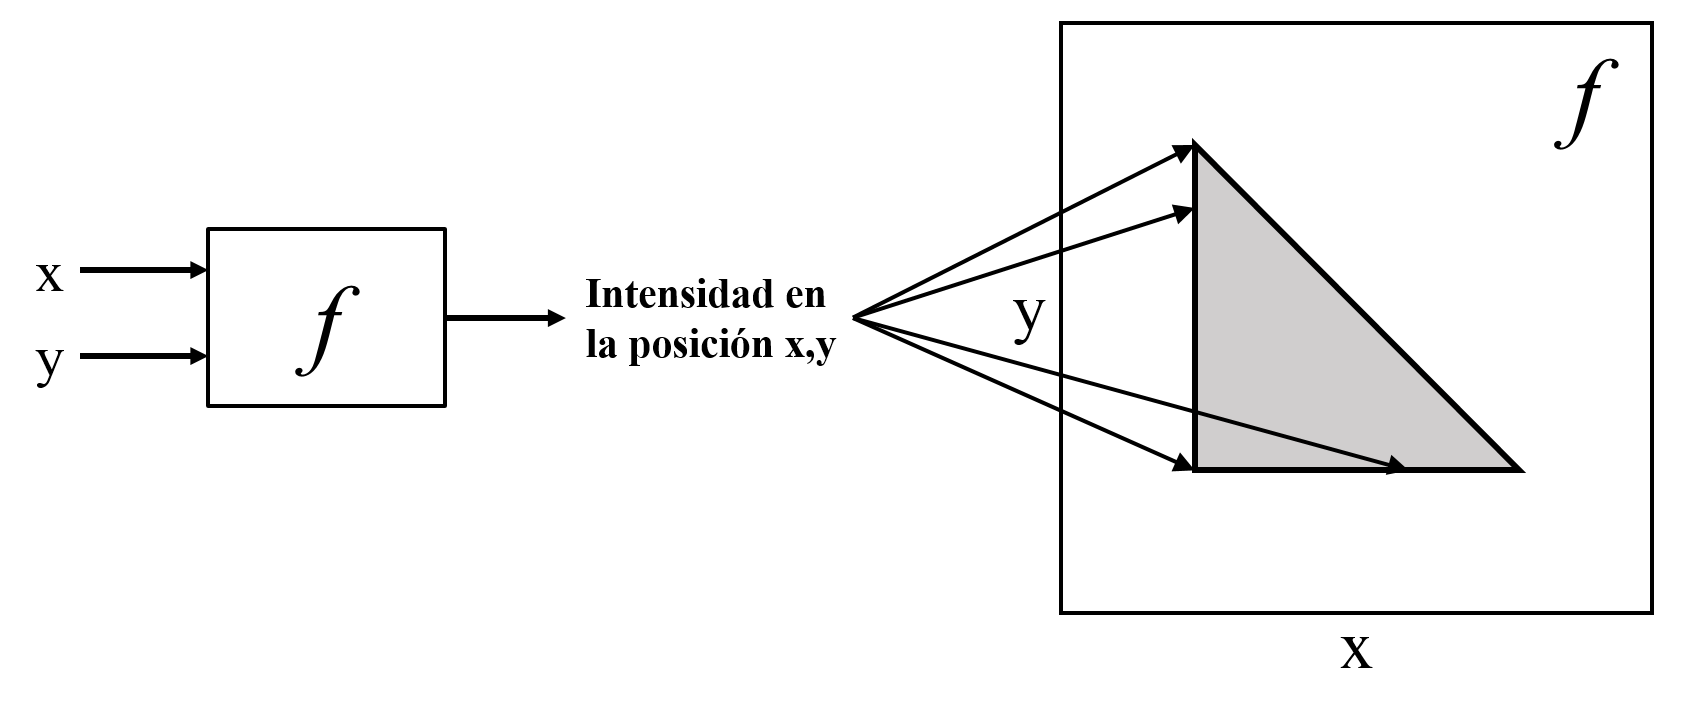
\includegraphics[width=0.8\textwidth]{fig/mapfenotipo.png}
\caption{\textbf{Una funci�n produce un fenotipo. } La funci�n \textit{f} toma los argumentos \textit{x} e \textit{y}, las cuales son coordenadas en un espacio bidimensional. Cuando todas las coordenadas son dibujadas con una intensidad correspondiente a la salida de la funci�n \textit{f}, el resultado es un patr�n, el cual puede ser visto como un fenotipo cuyo genotipo es \textit{f}. En este ejemplo, \textit{f} produce un fenotipo triangular.}
\label{mapfenotipo}
\end{figure}

Considere una distribuci�n de puntos o marco de coordenadas en un eje cartesiano de izquierda a derecha, donde la concentraci�n de puntos aumenta hacia la derecha. Las coordenadas de estos puntos a lo largo del eje podr�an estar definidas simplemente por una funci�n $f(x)=x$. Si consideramos una distribuci�n de puntos en donde estos estuvieran concentrados hacia el punto medio entre ambos extremos y que disminuyen su concentraci�n a medida que se acercan a los extremos, tal como se presentar�a una simetr�a bilateral, esta podr�a ser descrita simplemente como una funci�n Gaussiana $g(x) = \dfrac{1}{\sigma \sqrt{2\pi}}e^{-(x-\mu)^{2}/2 \sigma^{2}}$. Si se quisiera representar segmentaci�n, podr�a hacerse a trav�s de funciones peri�dicas. La funci�n $h(x) = sin(x)$ podr�a representar puntos repetidos de forma equidistante a lo largo de un eje de coordenadas.

Diferentes marcos de coordenadas podr�an interactuar en el proceso de desarrollo para producir patrones con regularidades mas complejas. Del mismo modo, marcos representados por funciones pueden interactuar y componer regularidades complejas. Por ejemplo, una simetr�a bilateral con segmentaci�n a lo largo de un eje de coordenadas de izquierda a derecha puede producir dos grupos de segmentos con polaridades opuestas. Esta distribuci�n podr�a ser representada f�cilmente poniendo como entrada de una funci�n peri�dica la salida de una funci�n sim�trica, realizando una composici�n de funciones, como se muestra en la figura \ref{compfunciones}. As� tambi�n, una serie de composiciones de funciones pueden unirse para formar una nueva composici�n de manera de producir marcos de coordenadas mas elaborados.

\begin{figure}[t]
\centering
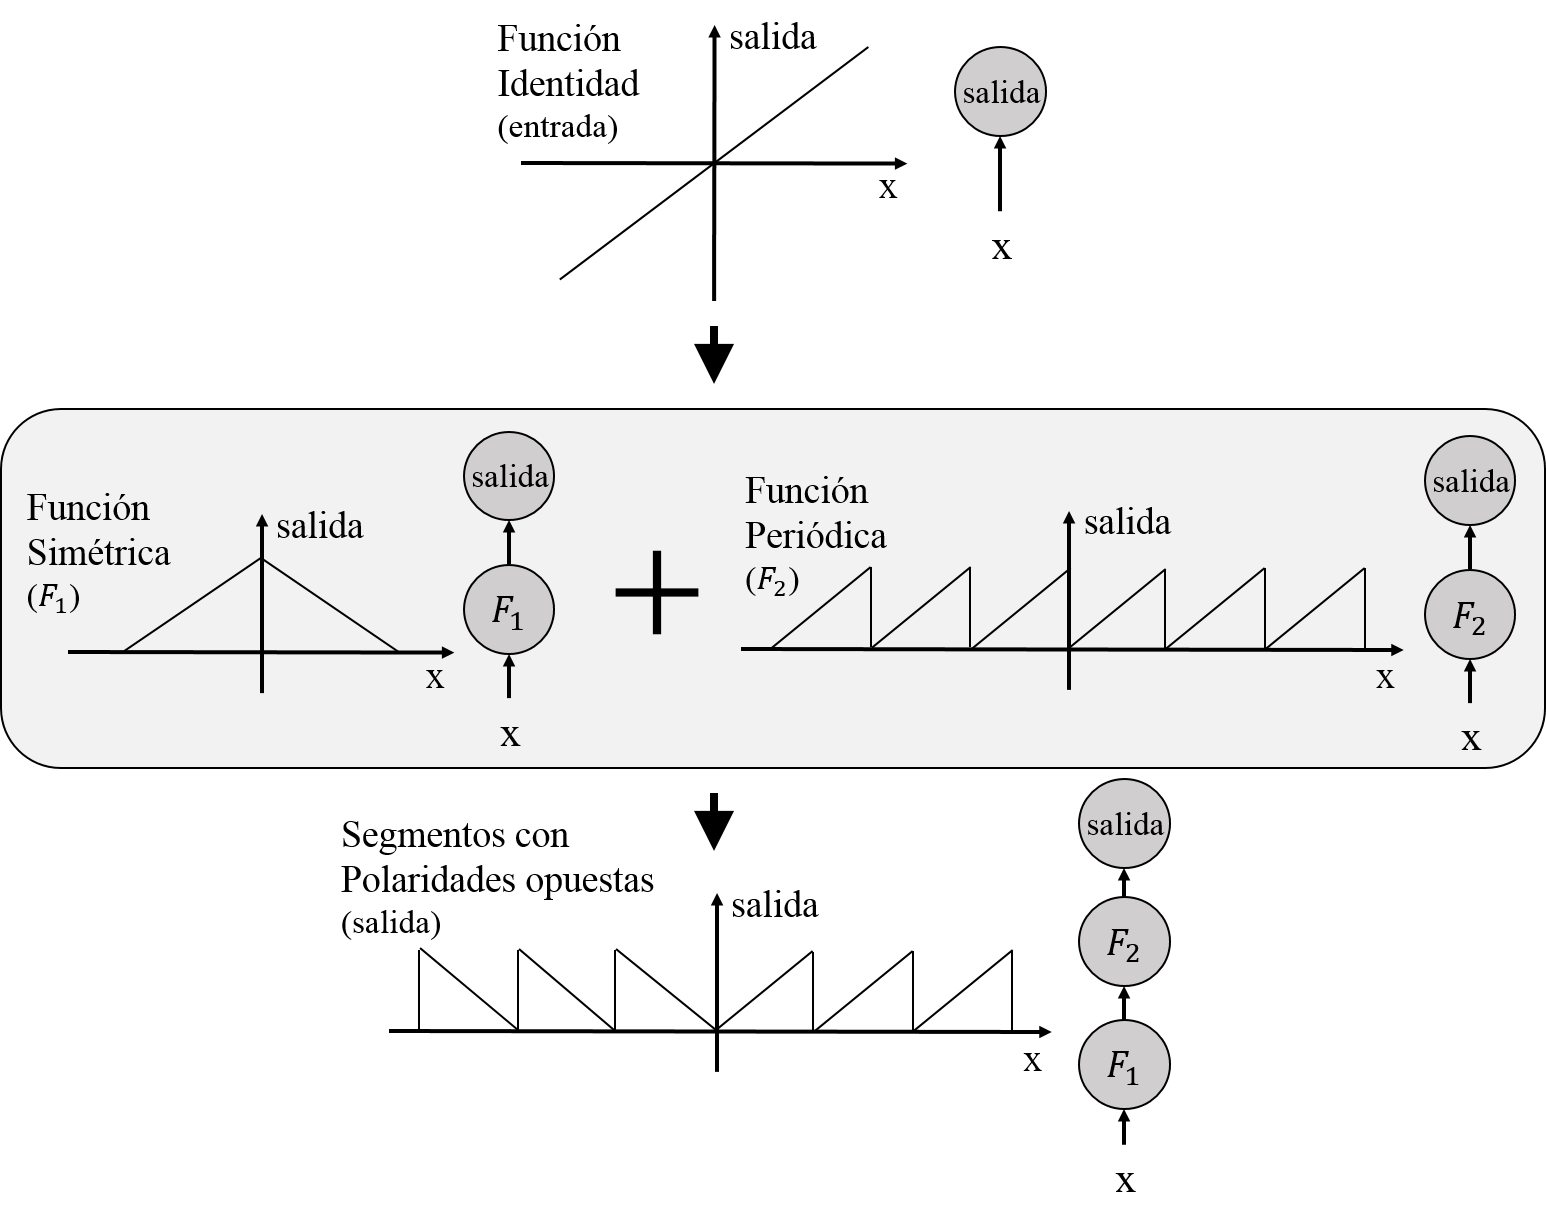
\includegraphics[width=0.8\textwidth]{fig/compfunciones.png}
\caption{\textbf{Composici�n de funciones. } Este ejemplo ilustra como una simple composici�n de funciones en una dimensi�n puede producir patrones con m�ltiples regularidades. Una representaci�n en forma de red de cada composici�n es mostrada a la derecha de los gr�ficos de cada funci�n. La entrada asim�trica inicial $x$ a la entrada de una composici�n de una funci�n sim�trica ($F_{1}$) y una funci�n peri�dica ($F_{2}$) produce dos grupos de segmentos con polaridades opuestas.}
\label{compfunciones}
\end{figure}

``Compositional Pattern Producing Networks'' (CPPNs) es un m�todo de codificaci�n que permite describir directamente relaciones estructurales de una topolog�a a trav�s de una composici�n de 		funciones. 

Una manera natural de representar una composici�n de funciones es a trav�s de un grafo de funciones interconectadas, como se muestra en la figura \ref{grafo}. Es as� como el sistema de coordenadas inicial de una estructura puede ser provisto como entrada del grafo. El siguiente nivel de nodos puede ser visto como una descripci�n inicial del primer sistema de coordenadas de dicha estructura. Niveles mas elevados de nodos establecer�n sistemas de coordenadas cada vez m�s refinados. Finalmente las salidas finales corresponder�n a las transformaciones de todas las capas anteriores, entregando una codificaci�n del sistema de coordenadas provisto.

\begin{figure}[t]
\centering
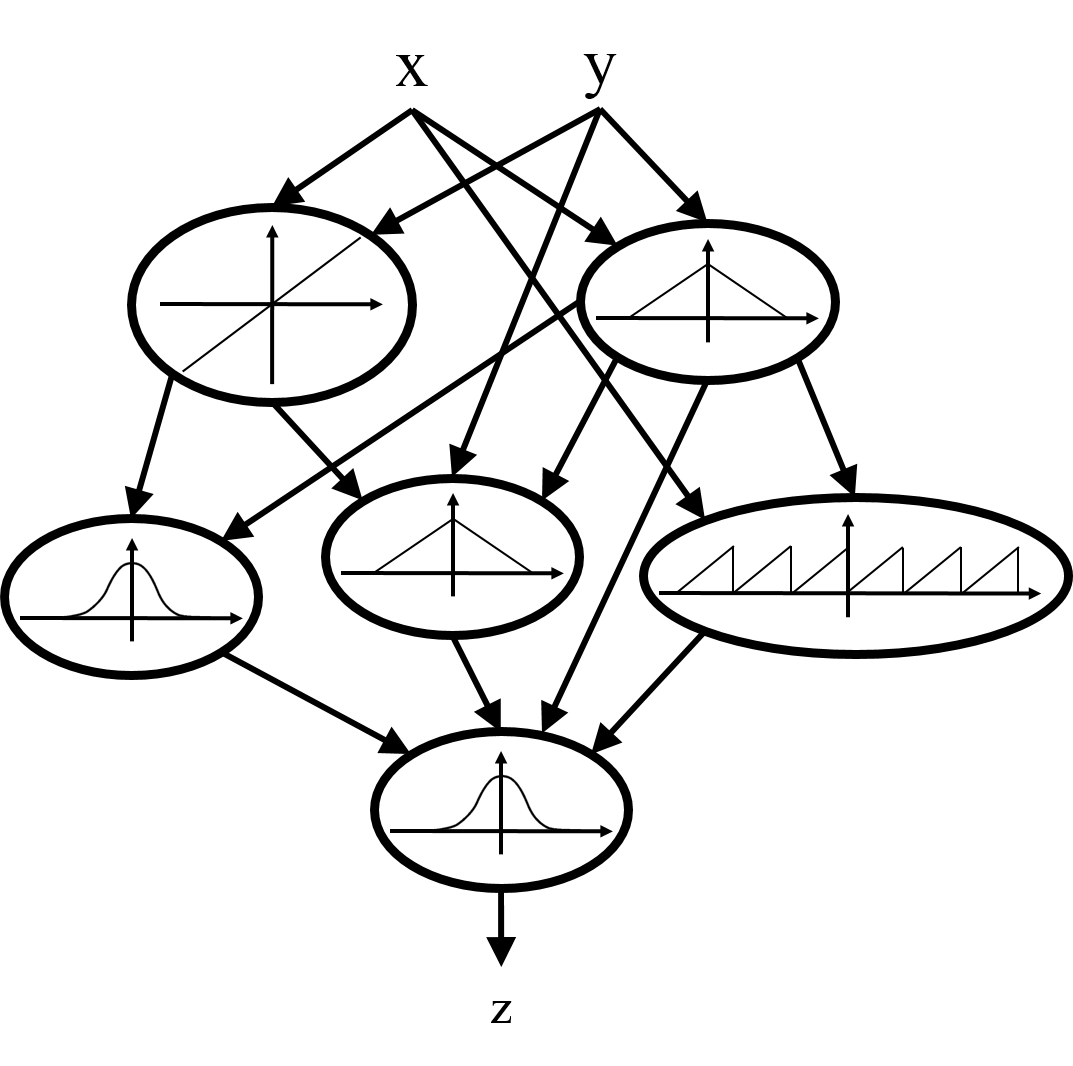
\includegraphics[width=0.5\textwidth]{fig/grafo.png}
\caption{\textbf{Composici�n de funciones en forma de grafo. } El grafo determina cual funci�n esta conectada con cual. A cada conexi�n se le asigna un peso, el cual multiplica a la salida de la funci�n del nodo entrante. Si m�ltiples conexiones entran a una misma funci�n, esta recibe como entrada la suma de las salidas de cada una de las funciones entrantes multiplicadas por sus respectivos pesos de conexi�n. Se debe tener en cuenta que la topolog�a no tiene restricciones y puede representar cualquier relaci�n posible. Esta representaci�n es similar al formalismo de las ANNs tradicionales con funciones de activaci�n y topolog�as arbitrarias.}
\label{grafo}
\end{figure}

Es interesante observar que un grafo de dicha composici�n es muy similar a una ANN con topolog�a arbitraria. La �nica diferencia entre ambas es que las ANNs generalmente usan funciones sigmoides (y a veces funciones Gaussianas) como funci�n de activaci�n de cada nodo, mientras que un grafo puede usar cualquier variedad de funciones can�nicas en cada nodo.

Finalmente podemos referirnos a ``Compositional Pattern Producing Networks'' (CPPNs) para describir una composici�n de funciones en forma de grafo que busca reproducir patrones regulares.

\subsection{EVOLUCIONANDO CPPNs}

Casualmente CPPNs y ANNs son pr�cticamente lo mismo desde una perspectiva estructural. Muchos m�todos para evolucionar topolog�as y pesos de conexi�n en ANNs ya existen, por lo que es posible extender de manera f�cil estos m�todos para evolucionar CPPNs a�adiendo peque�os cambios. Tambi�n hay m�todos para evolucionar programas gen�ticos, los cuales pueden ser muy similares a CPPNs.

Anteriormente se describi� una propiedad esencial de la evoluci�n en la naturaleza que describe la gradual complejizaci�n del genoma. La idea principal es iniciar con un peque�o genoma al cual se le a�aden nuevos genes en el trascurso de la evoluci�n. En CPPNs esto significa que se a�adir�n nuevas conexiones o nodos de funciones a la red, permitiendo as� complejizar la red para poder establecer regularidades fundamentales en los principios de su desarrollo para luego hacerlas m�s elaboradas a lo largo de la evoluci�n.

El m�todo a usar para evolucionar las CPPNs ser� ``NeuroEvolution of Augmenting Topologies'' (NEAT). NEAT es capaz de evolucionar ANNs incre�blemente complejas a lo largo de generaciones, y sobrellevar los desaf�os que conlleva evolucionar una gran poblaci�n de redes de diversas topolog�as mediante el uso de marcas hist�ricas. Ya que NEAT comienza trabajando sobre redes peque�as y solo expande su espacio de soluci�n cuando logra un beneficio de esta expansi�n, se vuelve capaz de encontrar ANNs significativamente m�s complejas, de forma contraria a m�todos que evolucionan topolog�as fijas.

A pesar de que NEAT originalmente fue dise�ado para evolucionar ANNs, solo se requiere de peque�as modificaciones para evolucionar CPPNs, ya que como se mencion�, estas son muy similares.

\section{NEAT}

Esta secci�n explica el fundamento del m�todo de neuroevoluci�n NEAT, su funcionamiento, y como este puede evolucionar CPPNs.

A diferencia de muchos otros m�todos para evolucionar ANNs (m�todos de neuroevoluci�n) existentes que tradicionalmente evolucionan redes con topolog�as fijas o generadas arbitrariamente de forma aleatoria, NEAT es la primera que inicia la evoluci�n a partir de una poblaci�n de peque�as y simples redes neuronales, aumentando su complejidad a lo largo de las generaciones, destacando un comportamiento cada vez m�s sofisticado.

Antes de describir como extender el algoritmo NEAT para evolucionar CPPNs es necesario describir las tres ideas principales de las cuales NEAT se basa. Primero, con el fin de permitir que las estructuras de las redes se vuelvan m�s complejas a trav�s de las generaciones, se hace necesario un m�todo para realizar un seguimiento de qu� gen es cu�l. De otra forma no es claro en posteriores generaciones cu�l individuo es compatible con cual, o c�mo estos genes pueden ser combinados para producir genes hijos. NEAT soluciona este problema asignando una marca hist�rica �nica a cada nueva pieza de la estructura de la red que aparezca a trav�s de mutaciones estructurales. La marca hist�rica es un n�mero asignado a cada gen correspondiente a su orden de aparici�n durante el curso de la evoluci�n. Estos n�meros son heredados durante el entrecruzamiento sin cambios, y permitiendo a NEAT realizar entrecruzamientos de genes sin la necesidad de un costoso an�lisis topol�gico. De esta forma, genomas con diferentes estructuras o tama�os mantienen la compatibilidad a lo largo de la evoluci�n, solucionando el problema planteado anteriormente de comparaci�n de diferentes topolog�as en una poblaci�n en evoluci�n.

Segundo, NEAT separa en especies a los individuos de una poblaci�n, por lo que los organismos compiten principalmente dentro de sus propios nichos en lugar de con toda la poblaci�n. De esta manera las innovaciones topol�gicas en los genes son protegidas y se les da tiempo para que optimicen sus estructuras antes de competir con otros nichos dentro de la poblaci�n. NEAT utiliza las marcas hist�ricas en genes para determinar a qu� especies pertenecen diferentes individuos.

Tercero, otros sistemas que evolucionan redes con topolog�as con nodos interconectados con pesos o costos en sus conexiones comienzan una evoluci�n con una poblaci�n con topolog�as aleatorias.  NEAT al contrario, comienza con una poblaci�n uniforme de redes simples sin capas intermedias, difiriendo solo en los pesos de sus conexiones inicializados aleatoriamente. Diversas topolog�as se acumulan gradualmente durante la evoluci�n, lo que permite diversos y complejos patrones fenot�picos para ser representados. No est� indicado un l�mite del tama�o que puede llegar a alcanzar una topolog�a. As�, NEAT puede iniciar la evoluci�n desde una estructura m�nima, y aumentar su tama�o sobre un n�mero determinado de generaciones.

Nuevas estructuras son introducidas como sucesos de mutaciones estructurales, y solo sobrevivir�n si es que resultan ser beneficiosas a trav�s del c�lculo de su desempe�o. De este modo, otra ventaja de la complejizaci�n es que NEAT busca a trav�s de soluciones dimensionalmente mas peque�as, reduciendo significativamente el n�mero de generaciones necesarias para encontrar la soluci�n, y asegurando que la red no se volver� mas compleja de lo necesario. En efecto, entonces, NEAT realiza una b�squeda de una soluci�n compacta y apropiada a trav�s del incremento de la complejidad de estructuras ya existentes.

\section{CPPN-NEAT}

CPPN-NEAT es una extensi�n de NEAT que permite evolucionar CPPNs. Mientras que redes en el m�todo NEAT original solo inclu�an nodos intermedios con funciones de activaci�n sigmoides, los nodos en CPPN-NEAT son creados asign�ndoles aleatoriamente una funci�n de activaci�n proveniente de un grupo can�nico determinado de funciones (que incluye por ejemplo la funci�n Gaussiana, Sigmoide, y funciones peri�dicas). Adem�s se define la funci�n de distancia de compatibilidad para determinar si dos redes pertenecen a la misma especie, la cual incluye la informaci�n de por cuantas funciones de activaci�n difieren dos individuos distintos. Esta caracter�stica permite que en la separaci�n de individuos en especies se tome en cuenta el n�mero de funciones de activaci�n que difieren entre individuos. Ya que CPPN-NEAT es una mejora de un preexistente efectivo m�todo de neuroevoluci�n, proporciona una base fiable para el estudio de la evoluci�n de formas cada vez mas complejas, como ANNs de gran escala o otras estructuras tipo grafo con simetr�as y patrones complejos de repetici�n. La siguiente secci�n presenta un enfoque que permite a CPPN representar y evolucionar simplemente este tipo de redes.

\section{HYPERNEAT}

Si CPPNs son evolucionadas para representar patrones de conectividad, el problema se dirige en encontrar la mejor interpretaci�n de sus salidas para describir efectivamente la estructura que se intenta representar. EL patr�n de dos dimensiones mostrado en la figura \ref{mapfenotipo} presenta un desaf�o: � C�mo pueden patrones espaciales describir la conectividad de una red ? Esta secci�n explica como patrones espaciales generados por CPPNs pueden mapear de manera natural patrones de conectividad de una red mientras que al mismo tiempo dan soluci�n a problemas asignados a dicha red desde su propia dimensionalidad.

\subsection{MAPEANDO PATRONES ESPACIALES A PATRONES DE CONECTIVIDAD}

Existe un mapeao eficaz entre los patrones espaciales y de conectividad que pueden elegantemente explotar las geometr�as de las estructuras. La idea principal es entregar a la entrada de una red CPPN las coordenadas de dos puntos que definan una conexi�n en lugar de entregar solo la posici�n de un �nico punto como se mostr� en la figura \ref{mapfenotipo}. La salida de la red CPPN es interpretado como el \textsl{peso} de la conexi�n en lugar de la intensidad de un punto. De esta formas las conexiones pueden ser definidas en t�rminos de la ubicaci�n de sus nodos terminales, teniendo as� en cuenta la geometr�a de la red.

CPPN en efecto calcula una funci�n $\text{CPPN}(x_{1}, y_{1}, x_{2}, y_{2})=\omega$ de cuatro dimensiones, en donde el primer nodo se encuentra en la coordenada $(x_{1}, y_{1})$ y el segundo en $(x_{2}, y_{2})$. A partir de esta funci�n se retorna el peso de cada una de las conexiones entre cada nodo en la red. Por convenci�n, una conexi�n no se realiza si la magnitud del peso resultante de la funci�n $\text{CPPN}$, que puede ser positiva o negativa, se encuentra por debajo de un umbral m�nimo $\omega_{min}$. Las magnitudes de los pesos por sobre este umbral son escalados entre cero y una magnitud m�xima $\omega_{max}$, definida para cada red como uno sobre el n�mero de nodos de la capa formada por el menor n�mero de ellos. De esta forma, los patrones producidos por la red CPPN pueden representar cualquier topolog�a de red.

Por ejemplo, considere una malla de $5 \times 5$ nodos. A cada nodo se le asigna una coordenada correspondiente a la posici�n de este dentro de la malla (nombrada como \textsl{substrato} en la figura \ref{hyperneat}), donde la coordenada $(0,0)$ corresponde al centro de la malla. Asumiendo que estos nodos y sus posiciones son dadas \textsl{a priori}, un patr�n de conectividad entre nodos en un espacio bidimensional es producido por una red CPPN que toma dos coordenadas (fuente y destino) como entrada, y que retorna como salida el peso de la conexi�n entre estos nodos. La red CPPN calcula de esta manera entonces cada conexi�n potencial en la malla. Ya que los pesos de las conexiones son de un modo una funci�n de las posiciones de los nodos de fuente y destino, la distribuci�n de pesos en las conexiones a lo largo de la malla exhibir� un patr�n que estar� en funci�n de la geometr�a del sistema de coordenadas de la malla.

El patr�n de coordenadas producido por una red CPPN ser� llamado \textsl{substrato} de forma de distinguirlo verbalmente de la red CPPN misma, el cual tendr� su propia topolog�a interna.

\begin{figure}[t]
\centering
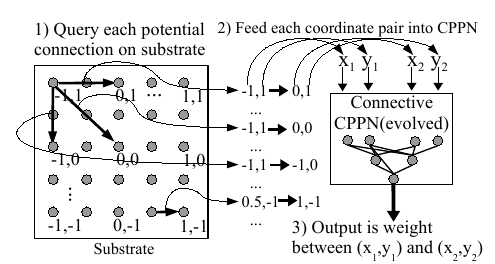
\includegraphics[width=0.8\textwidth]{fig/hyperneat.png}
\caption{\textbf{Interpretaci�n del patr�n geom�trico de conectividad de un hipercubo. } En una malla de nodos, llamada \textsl{substrato}, a cada uno de los nodos se le es asignada una coordenada tal que el nodo central se encuentra en el origen. (1) Cada conexi�n potencial es consultada para determinar si esta existe, y de existir, cual ser�a su peso; la linea negra en la parte inferior derecha del substrato indica una posible conexi�n a ser consultada. (2) Por cada consulta, la red CPPN toma como entrada las coordenadas de los dos puntos terminales y (3) entrega como salida el peso de la conexi�n entre ellos. Luego de que todas las conexiones han sido determinadas, un patr�n de conexiones y pesos de conexi�n resultan en funci�n de la geometr�a del substrato. De esta forma, la red CPPN produce patrones de regularidad de conexiones en el espacio.}
\label{hyperneat}
\end{figure}

Ya que la red CPPN en este caso representa una funci�n de cuatro dimensiones, el patr�n de conectividad bidimensional expresado por la red CPPN es isomorfo al patr�n espacial presente en un hipercubo de cuatro dimensiones. Esta observaci�n es importante ya que esto significa que patrones espaciales con simetr�as y regularidades corresponden a patrones de conectividad tambi�n con dichas simetr�as y regularidades. As�, tal como CPPNs generan patrones espaciales regulares, por extensi�n se puede esperar que puedan producir patrones de conectividad con las correspondientes regularidades. La siguiente secci�n muestra dichas capacidades.

\subsection{GENERACI�N DE PATRONES DE CONECTIVIDAD REGULARES}

Subestructuras descubiertas en la red CPPN producen importantes regularidades en las conexiones del substrato utilizando como entradas los valores de las coordenadas de los puntos en el eje $x$ y en el eje $y$. As� por ejemplo, una simetr�a a lo largo del eje $x$ puede ser simplemente descubierta mediante la aplicaci�n de una funci�n sim�trica (por ejemplo Gaussiana) a las coordenadas $x_{1}$ y $x_{2}$ (figura \ref{fig:patronsim}).

\begin{figure}[t]
	\centering
	\begin{subfigure}[b]{0.35\textwidth}
		\centering
        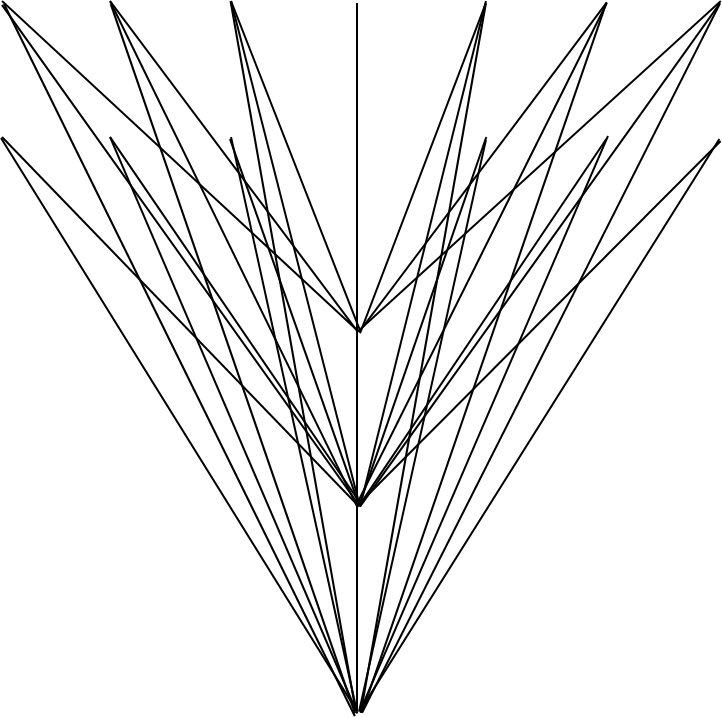
\includegraphics[width=0.7\textwidth]{fig/patronescppn1.png}
        \caption{Simetr�a}
        \label{fig:patronsim}
    \end{subfigure}
    ~
    \begin{subfigure}[b]{0.35\textwidth}
    	\centering
        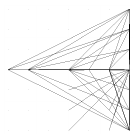
\includegraphics[width=0.7\textwidth]{fig/patronescppn2.png}
        \caption{Simetr�a Imperfecta}
        \label{fig:patronsimimp}
    \end{subfigure}
    
    \begin{subfigure}[b]{0.35\textwidth}
    	\centering
        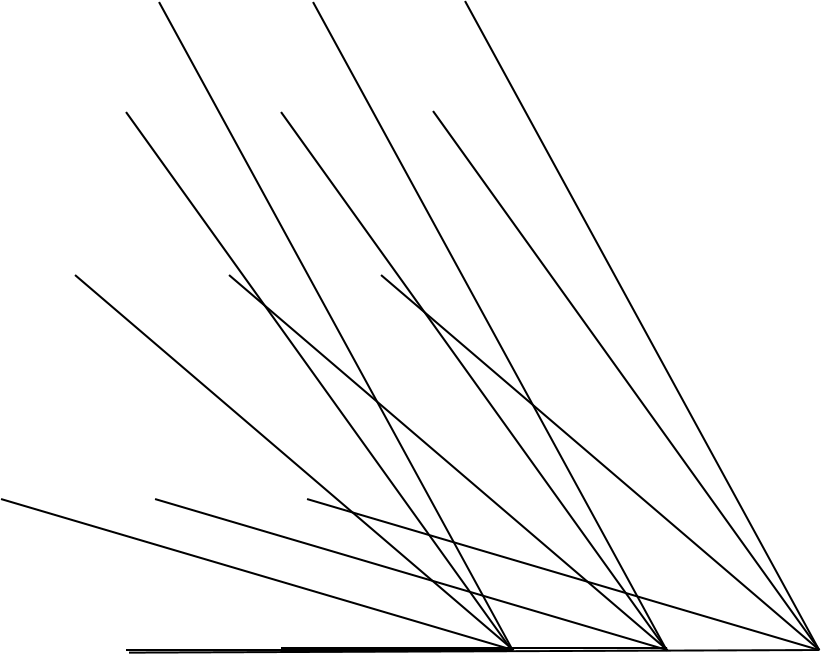
\includegraphics[width=0.7\textwidth]{fig/patronescppn3.png}
        \caption{Repetici�n}
        \label{fig:patronrep}
    \end{subfigure}
    ~ 
    \begin{subfigure}[b]{0.35\textwidth}
    	\centering
        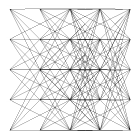
\includegraphics[width=0.7\textwidth]{fig/patronescppn4.png}
        \caption{Repetici�n con Variaciones}
        \label{fig:patronrepvar}
    \end{subfigure}
    \caption{\textbf{Patrones de conectividad producidos por CPPNs. } Estos patrones, producidos a trav�s de la evoluci�n, exhiben importantes casos de patrones de conectividad: (a) simetr�a bilateral, (b) simetr�a imperfecta, (c) repetici�n, y (d) repetici�n con variaciones. Que estos patrones sean generados f�cilmente y representados de forma compacta sugiere el poder de esta codificaci�n.}
    \label{fig:patronescppn}
\end{figure}

Una simetr�a imperfecta es otro importante patr�n observado. Una red CPPN puede producir simetr�as imperfectas por la composici�n de dos funciones sim�tricas junto a un marco de coordenadas asim�trico. De esta manera, la red CPPN puede producir diferentes grados de simetr�as imperfectas como el ejemplo de la figura \ref{fig:patronsimimp}.

Otro patr�n importante es el de repetici�n, particularmente el de repetici�n con variaciones. Tal como funciones sim�tricas producen simetr�as, funciones peri�dicas, como la funci�n seno, produce repeticiones (figura \ref{fig:patronrep}). Patrones con variaciones son producidos por una composici�n de una funci�n peri�dica con un marco de coordenadas sin repeticiones, tal como su propio eje (figura \ref{fig:patronrepvar}). As�, simetr�a, simetr�a imperfecta, repetici�n y repetici�n con variaciones son regularidades que pueden ser representadas de forma compacta y por lo tanto f�cilmente descubiertas por CPPNs.

La siguiente secci�n ahondar� en las configuraciones que puede adoptar el substrato.

\subsection{CONFIGURACIONES DEL SUBSTRATO}

La disposici�n de los nodos que CPPN conecta en el substrato puede tomar otras formas distintas a la malla plana mostrada en el ejemplo demostrativo de la figura \ref{hyperneat} y en la figura \ref{fig:substrateconf1}. Configuraciones de substratos diferentes son probablemente m�s adecuadas para distintos tipos de problemas.

\begin{figure}[t]
	\centering
	\begin{subfigure}[b]{0.35\textwidth}
		\centering
        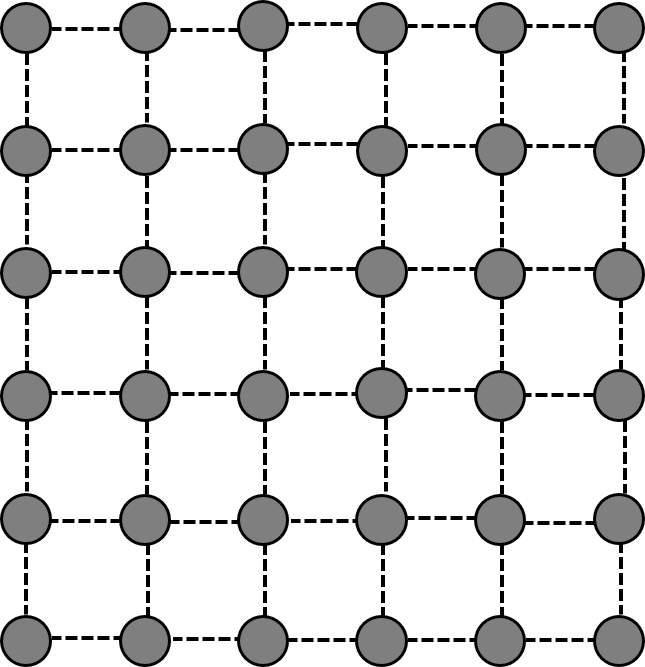
\includegraphics[width=0.7\textwidth]{fig/substrateconf1.png}
        \caption{Maya}
        \label{fig:substrateconf1}
    \end{subfigure}
    ~
    \begin{subfigure}[b]{0.35\textwidth}
    	\centering
        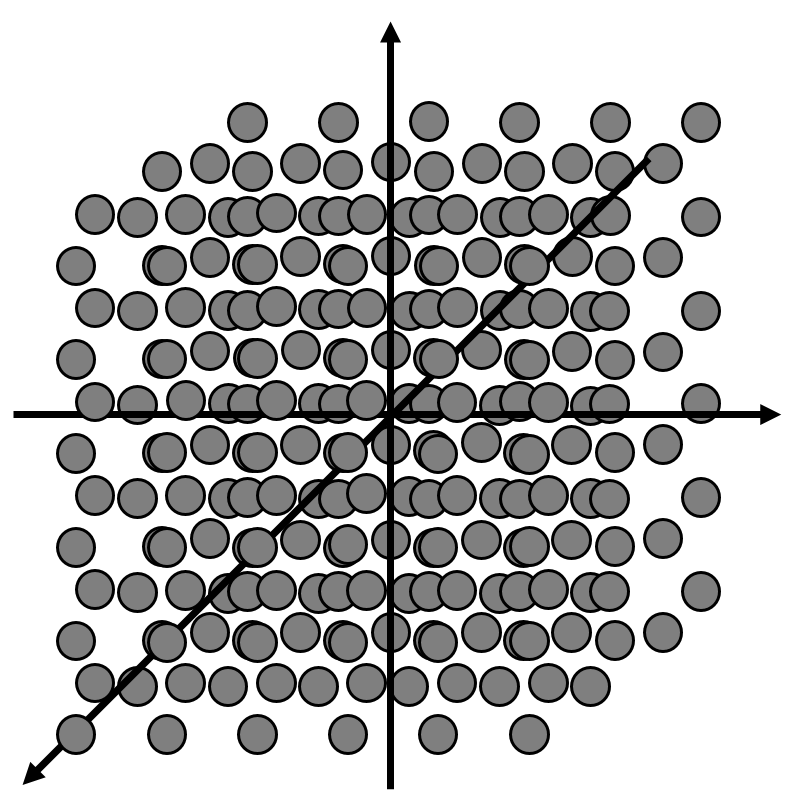
\includegraphics[width=0.7\textwidth]{fig/substrateconf2.png}
        \caption{Tridimensional}
        \label{fig:substrateconf2}
    \end{subfigure}
    
    \begin{subfigure}[b]{0.35\textwidth}
    	\centering
        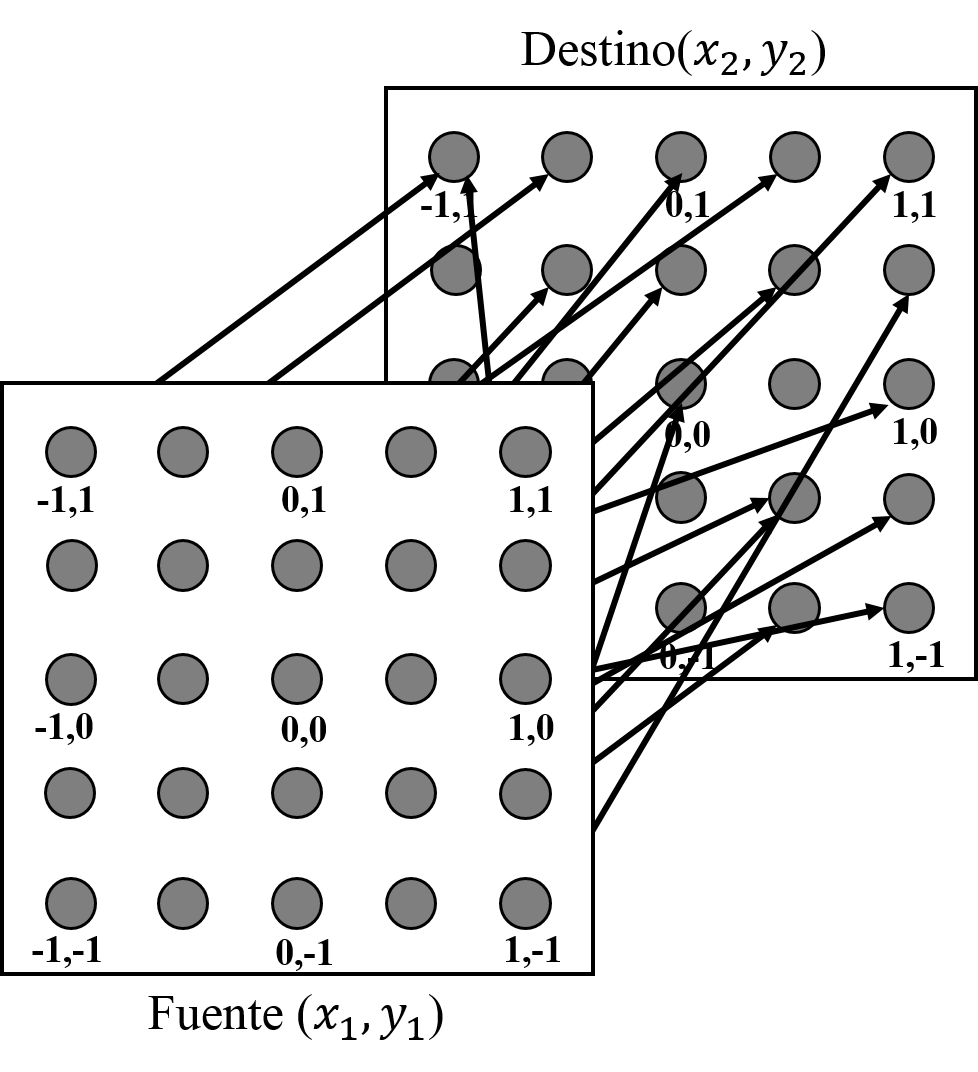
\includegraphics[width=0.7\textwidth]{fig/substrateconf3.png}
        \caption{S�ndwich}
        \label{fig:substrateconf3}
    \end{subfigure}
    ~ 
    \begin{subfigure}[b]{0.35\textwidth}
    	\centering
        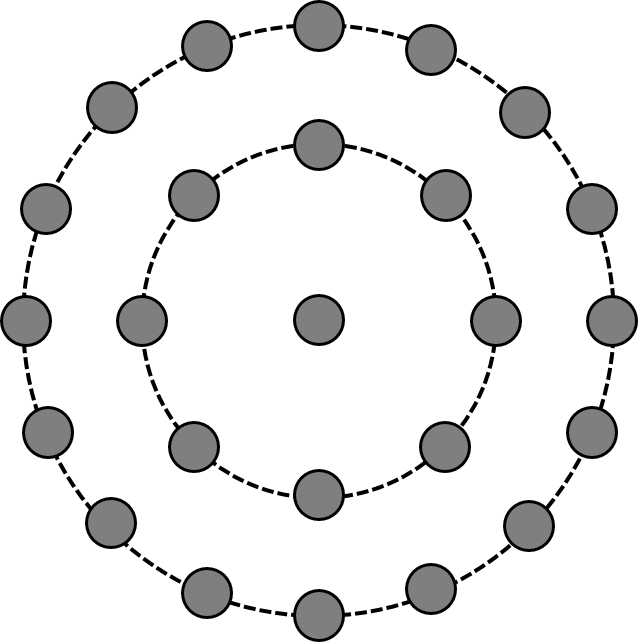
\includegraphics[width=0.7\textwidth]{fig/substrateconf4.png}
        \caption{Circular}
        \label{fig:substrateconf4}
    \end{subfigure}
    \caption{\textbf{Alternativas de configuraci�n del Substrato. } Estas figuras muestran (b) una configuraci�n tridimensional de nodos centrados en (0,0,0), (c) una configuraci�n s�ndwich de dos capas en la cual una capa fuente de neuronas se conecta directamente a una capa destino, y (d) una configuraci�n circular. Diferentes configuraciones son probablemente mas adecuadas para problemas con diferentes propiedades geom�tricas.}
    \label{fig:substrateconf}
\end{figure}

Por ejemplo, CPPNs tambi�n pueden producir patrones de conectividad tridimensionales por la representaci�n espacial de patrones de la funci�n $\text{CPPN}(x_{1},y_{1},z_{1},x_{2},y_{2},z_{2})$ en un hipercubo de seis dimensiones (figura \ref{fig:substrateconf2}), tal como es te�ricamente la topolog�a de los cerebros biol�gicos.

Tambi�n es posible restringir configuraciones de substrato a determinadas topolog�as con el fin de aprender acerca de su viabilidad de forma aislada. Por ejemplo, Churchland \cite{churchuland} llama a una simple capa bidimensional de neuronas conectada a otra capa bidimensional un \textit{``state-space sandwich''}. El s�ndwich es una estructura tridimensional restringida en la cual una capa solo puede entablar conexiones en una sola direcci�n hacia otra capa. Por lo tanto, debido a esta restricci�n, se puede expresar por una �nica funci�n $\text{CPPN}(x_{1},y_{1},x_{2},y_{2})$ de dimensi�n cuatro, donde $(x_{2},y_{2})$ se interpreta como una locaci�n en la capa de destino en lugar de estar en el mismo plano de coordenadas de $(x_{1},y_{1})$. De esta manera, CPPNs pueden hacer b�squeda de patrones �tiles dentro de un substrato con configuraci�n state-space sandwich (figura \ref{fig:substrateconf3}).

Finalmente, los nodos en una capa no tienen que estar necesariamente distribuidos en forma de malla. Por ejemplo, nodos dentro de un substrato que controla entradas radiales, como por ejemplo un robot con sensores de distancia situados a su alrededor, podr�an estar dispuestos mejor en un esquema con simetr�a radial, como se muestra en la figura \ref{fig:substrateconf4}, de modo que el patr�n de conectividad se pueda establecer con un sistema de coordenadas polares perfecto.

\subsection{POSICIONAMIENTO DE ENTRADAS Y SALIDAS}

Parte de la configuraci�n del substrato es la determinaci�n de cuales nodos son entradas y cuales salidas. La flexibilidad de asignar entradas y salidas a coordenadas especificas en el substrato crea una oportunidad de explorar relaciones geom�tricas ventajosamente.

En muchas aplicaciones de ANNs, las entradas son dibujadas por un grupo de sensores en un arreglo geom�trico en el espacio. A diferencia de los algoritmos tradicionales de aprendizaje de ANNs que no son conscientes de tal geometr�a, una red CPPN si sera consciente de ello y puede usar esa informaci�n a su favor.

Mediante la disposici�n de las entradas y las salidas en una configuraci�n especifica en el substrato, regularidades en la geometr�a pueden ser explotadas por la codificaci�n. Esto permite ser creativos para probar diferentes configuraciones geom�tricas que aporten distintas ventajas. Por ejemplo, la figura \ref{fig:posio} describe dos m�todos en los cuales las entradas y las salidas de un robot circular pueden ser configuradas, en donde ambas crean una oportunidad de explotar diferentes formas de relaciones geom�tricas. 

\begin{figure}[t]
	\centering
	\begin{subfigure}[b]{0.3\textwidth}
		\centering
        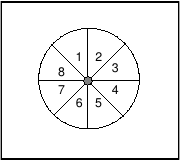
\includegraphics[width=\textwidth]{fig/posio1.png}
        \caption{Robot}
        \label{fig:posio1}
    \end{subfigure}
    ~
    \begin{subfigure}[b]{0.3\textwidth}
    	\centering
        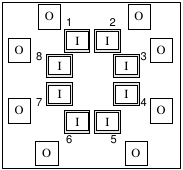
\includegraphics[width=\textwidth]{fig/posio2.png}
        \caption{Conc�ntrica}
        \label{fig:posio2}
    \end{subfigure}
    ~ 
    \begin{subfigure}[b]{0.3\textwidth}
    	\centering
        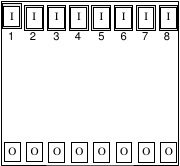
\includegraphics[width=\textwidth]{fig/posio3.png}
        \caption{Paralela}
        \label{fig:posio3}
    \end{subfigure}
    \caption{\textbf{Posicionando entradas y salidas. } Un robot (a) es descrito con ocho sensores lidar como entradas de est�mulos, y ocho actuadores para respuestas motoras situados de forma radial equiangularmente distanciados. En (b), las entradas (de etiqueta \textit{I}, correspondientes a sensores lidar) y salidas (de etiqueta \textit{O}, correspondientes a actuadores) est�n situadas en la misma diagonal en los ocho sectores indicados en (a). En (c), entradas y salidas son situadas horizontales y paralelamente unas de la otras en dos filas. Ambos arreglos crean una relaci�n geom�trica entre cada entrada y su correspondiente salida. De esta forma es posible dar ventaja a la evoluci�n desde el comienzo.}
    \label{fig:posio}
\end{figure}

En un arreglo, los sensores de la periferia del robot son situados en un circulo centrado en el origen del substrato, y las salidas forman una circunferencia conc�ntrica alrededor de este (figura \ref{fig:posio2}). De esta forma, si la red CPPN descubre simetr�as radiales o bilaterales, esta puede usar este sistema de coordenadas para crear un patr�n repetitivo que capture regularidades en las conexiones entre las entradas y las salidas. Un arreglo alternativo es situar las entradas y las salidas en dos lineas paralelas en donde la posici�n de cada entrada y salida esta correlacionada con el �ngulo de ubicaci�n en el robot en cada una de sus filas respectivamente (figura \ref{fig:posio3}). De esa forma, la evoluci�n puede explotar las similitudes de las posiciones horizontales de las entradas y salidas. Ambos m�todos representan correspondencia a trav�s de una regularidad geom�trica diferente.

A trav�s del arreglo de las neuronas en una configuraci�n especifica en el substrato, regularidades en la geometr�a pueden ser explotadas por la codificaci�n. 

\subsection{RESOLUCI�N DEL SUBSTRATO}

En contraposici�n con la codificaci�n de un patr�n espec�fico de conexiones entre un conjunto espec�fico de nodos, una red CPPN en efecto codifica un concepto de conectividad general, es decir, los fundamentos de las relaciones matem�ticas producen un patr�n particular. La consecuencia es que la misma red CPPN puede representar un concepto equivalente en diferentes resoluciones o densidades de nodos. La figura \ref{fig:substrateres} muestra dos conceptos de conectividad en diferentes resoluciones.

\begin{figure}[ht!]
	\centering
	\begin{subfigure}[b]{0.3\textwidth}
		\centering
        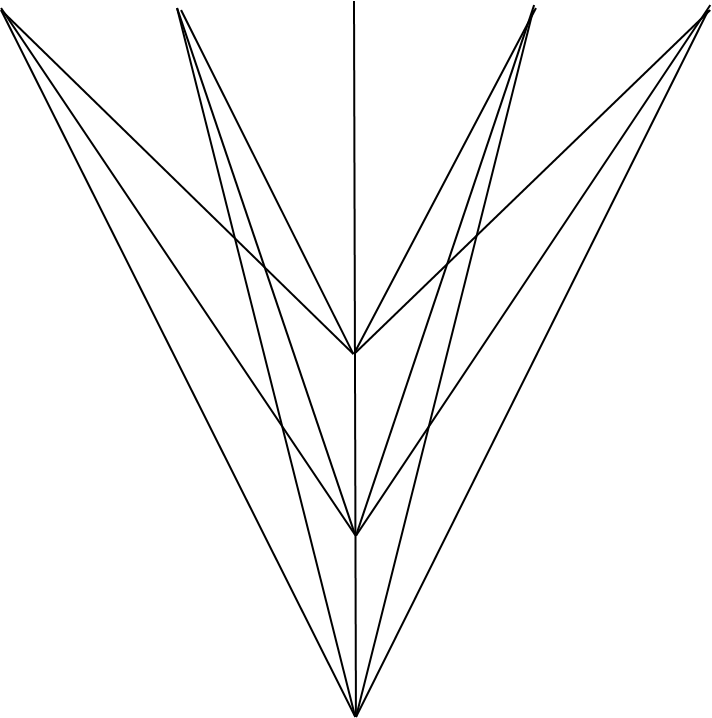
\includegraphics[width=\textwidth]{fig/substrateres1.png}
        \caption{Concepto 1 de $5 \times 5$}
        \label{fig:substrateres1}
    \end{subfigure}
    ~
    \begin{subfigure}[b]{0.3\textwidth}
    	\centering
        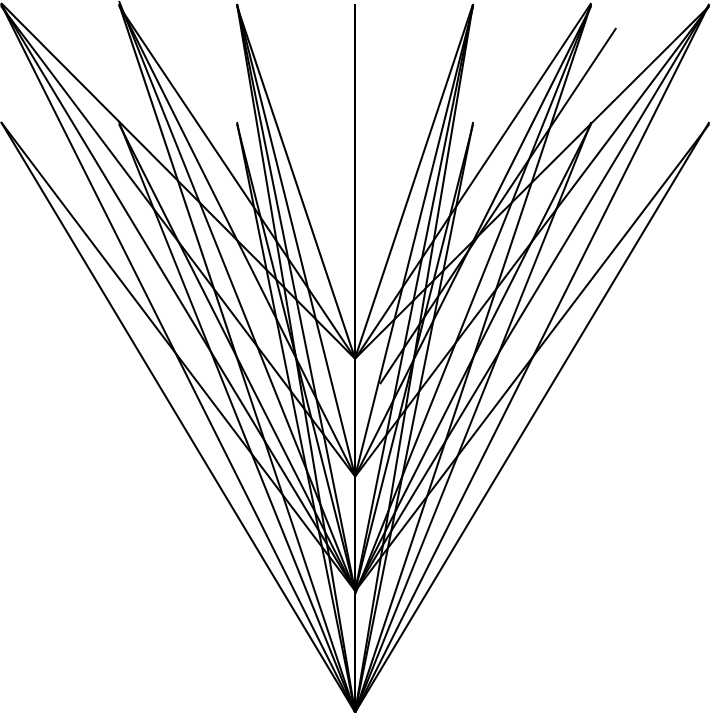
\includegraphics[width=\textwidth]{fig/substrateres2.png}
        \caption{Concepto 1 de $7 \times 7$}
        \label{fig:substrateres2}
    \end{subfigure}
    ~ 
    \begin{subfigure}[b]{0.3\textwidth}
    	\centering
        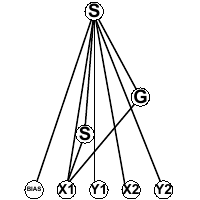
\includegraphics[width=\textwidth]{fig/substrateres3.png}
        \caption{Concepto 1 de CPPN}
        \label{fig:substrateres3}
    \end{subfigure}
    
    \centering
	\begin{subfigure}[b]{0.3\textwidth}
		\centering
        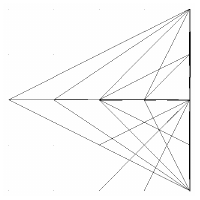
\includegraphics[width=\textwidth]{fig/substrateres4.png}
        \caption{Concepto 2 de $5 \times 5$}
        \label{fig:substrateres4}
    \end{subfigure}
    ~
    \begin{subfigure}[b]{0.3\textwidth}
    	\centering
        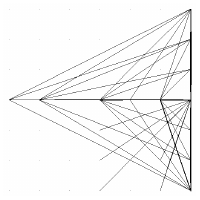
\includegraphics[width=\textwidth]{fig/substrateres5.png}
        \caption{Concepto 2 de $7 \times 7$}
        \label{fig:substrateres5}
    \end{subfigure}
    ~ 
    \begin{subfigure}[b]{0.3\textwidth}
    	\centering
        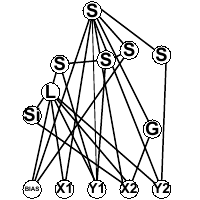
\includegraphics[width=\textwidth]{fig/substrateres6.png}
        \caption{Concepto 2 de CPPN}
        \label{fig:substrateres6}
    \end{subfigure}
    \caption{\textbf{Conceptos de conectividad equivalentes en diferentes resoluciones del substrato. } Se describen dos conceptos de conectividad generados en el proceso de evoluci�n. La red CPPN que genera el primer concepto a resoluciones de $5 \times 5$ (a) y $7 \times 7$ (b) es mostrado en (c). La red CPPN en (f) genera de forma similar el segundo concepto en ambas resoluciones (d) y (e). Esta ilustraci�n demuestra que CPPNs representan un concepto matem�tico en lugar de una sola estructura. As�, la misma red CPPN puede producir patrones con el mismo fundamento conceptual en diferentes resoluciones del substrato en diferente densidad de nodos. Las funciones de activaci�n de las redes CPPN mostradas est�n denotadas por \textit{G} para funciones \textit{Gaussianas}, \textit{S} para \textit{Sigmoides}, \textit{Si} para \textit{Senos}, y \textit{L} para \textit{Lineales}.}
    \label{fig:substrateres}
\end{figure}

Para substratos con neuronas, la importante implicancia de esto es que la misma funcionalidad de la ANN puede ser generada en distintas resoluciones. Sin m�s evoluci�n, una red CPPN previamente evolucionada puede ser usada para especificar el patr�n de conectividad de un mismo tipo de substrato con una resoluci�n mayor, generando de este modo una soluci�n para un mismo problema con una resoluci�n mas alta.  

\subsection{EVOLUCI�N DE LA RED CPPN}

La propuesta de este m�todo base para la implementaci�n de \(\tau\)-HyperNEAT es evolucionar una red CPPN usando NEAT para generar un patr�n de conectividad en otra red principal que posee caracter�sticas geom�tricas propias del problema a solucionar. Este m�todo base es llamado HyperNEAT ya que se usa a NEAT para evolucionar una red CPPN que busca representar patrones espaciales en un hiperespacio. Cada punto en el patr�n, delimitado por un hipercubo, es interpretado como una conexi�n en un grafo dimensionalmente m�s peque�o.

\clearpage

El esquema b�sico del algoritmo del m�todo HyperNEAT se muestra a continuaci�n:

\begin{enumerate}
\item Elegir una configuraci�n de substrato, es decir, el posicionamiento de cada nodo y la asignaci�n de nodos de entrada y salida.
\item Inicializar una poblaci�n de redes CPPN con pesos asignados de forma aleatoria.
\item Repetir hasta encontrar una soluci�n:
	\begin{enumerate}
	\item Por cada miembro de la poblaci�n de redes CPPN:
		\begin{enumerate}[label=(\roman*)]
		\item Usar la red CPPN para determinar el peso de cada posible conexi�n en el substrato. Si el valor absoluto de la salida de la red CPPN sobrepasa la magnitud de un umbral, se crea la conexi�n con el peso dado por la salida de la red CPPN escalada apropiadamente.
		\item Se usa el substrato como una ANN en la tarea a resolver para determinar su desempe�o y asignar el resultado a la red CPPN.
		\end{enumerate}
	\item Reproducir las redes CPPN acorde al m�todo NEAT para producir una nueva poblaci�n de CPPNs correspondientes a una nueva generaci�n.
	\end{enumerate}
\end{enumerate}

En efecto, como HyperNEAT incorpora nuevas conexiones y nodos a la estructura de la red CPPN, esta esta descubriendo nuevas dimensiones globales de variaciones en los patrones de conectividad a trav�s del substrato. Al principio es posible descubrir una simetr�a global, para luego descubrir un concepto mas elaborado de las regularidades del sistema. Cada nuevo nodo y conexi�n en el substrato representan una nueva manera en que un patr�n a generar pueda variar d�ndose nuevas regularidades. As�, HyperNEAT es una propuesta para evolucionar patrones de conectividad a gran escala en ANNs.

\chapter{$\tau$-HYPERNEAT}

Una vez comprendido el funcionamiento del m�todo de neuroevoluci�n HyperNEAT es posible extenderlo para implementar el m�todo \(\tau\)-HyperNEAT propuesto en esta memoria. \(\tau\)-HyperNEAT poseer� la misma estructura que su predecesor, con una configuraci�n definida del substrato y una poblaci�n inicial de organismos CPPN de topolog�a b�sica �nicamente diferenciados por la aleatoriedad de la asignaci�n de los pesos de sus conexiones. Sin embargo, la topolog�a b�sica inicial de estos organismos ser� diferente que para el caso de HyperNEAT. Adem�s de que una red CPPN entregue el peso como resultado de la consulta de una conexi�n entre dos nodos dentro del substrato, entregar� un segundo valor correspondiente al porcentaje de retardo (con respecto a un retardo m�ximo) asignado a la conexi�n entre dichos nodos. El retardo de conexi�n es implementado en el substrato por medio de un \textit{buffer}, el cual poseer� un largo proporcional al retardo.

La figura \ref{tauhyperneat} muestra un esquema del m�todo \(\tau\)-HyperNEAT propuesto, el cual es muy similar al esquema de la figura \ref{hyperneat}. Una red CPPN se encarga de generar un patr�n de conectividad entre todos los nodos ubicados en el substrato, tomando como entradas las coordenadas de los nodos (fuente y destino), y retornando el peso y el porcentaje de retardo en la conexi�n entre estos nodos. De esta forma, la red CPPN calcula entonces cada conexi�n potencial en el substrato. Tal como ocurre en el m�todo HyperNEAT en donde la distribuci�n de los pesos en las conexiones a lo largo del substrato exhibe un patr�n en funci�n de las geometr�as del sistema de coordenadas del substrato, los retardos tambi�n estar�n distribuidos en funci�n de este.

\begin{figure}[t]
\centering
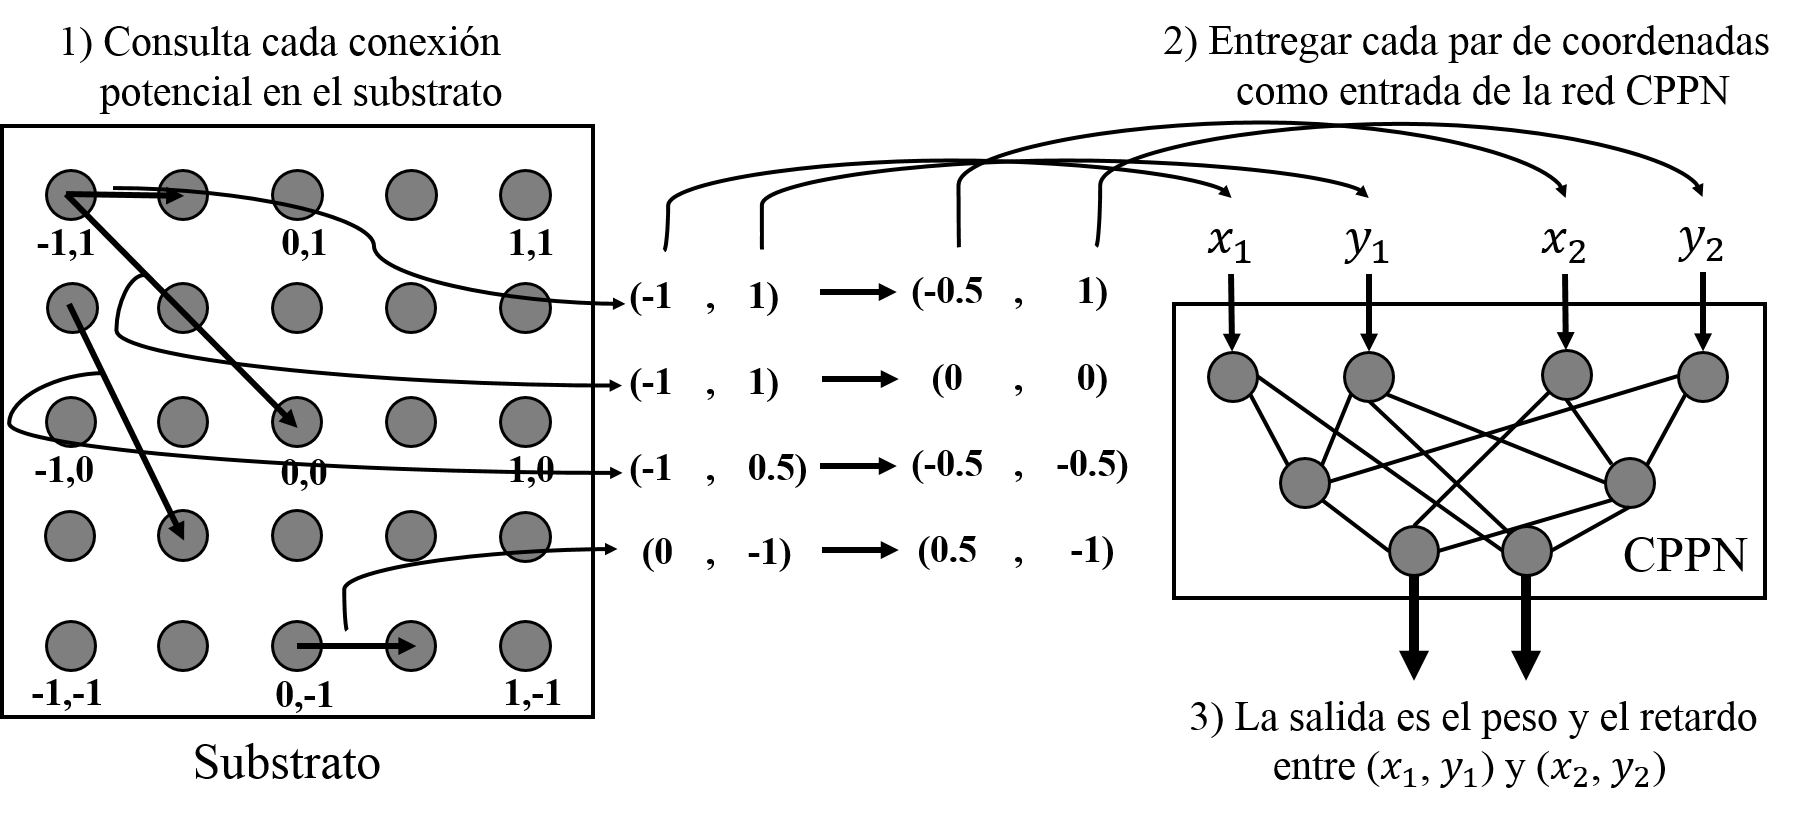
\includegraphics[width=0.8\textwidth]{fig/tauhyperneat.png}
\caption{\textbf{Interpretaci�n del patr�n geom�trico de conectividad de un hipercubo usando \(\tau\)-HyperNEAT. } Al igual que como funciona el m�todo HyperNEAT (1) cada conexi�n potencial es consultada para determinar si esta existe, y de existir, cual ser�a su peso y su retardo asociado. (2) Por cada consulta, la red CPPN toma como entrada las coordenadas de los dos puntos terminales y (3) entrega como salida el peso y el retardo de la conexi�n entre ellos. Luego de que todas las conexiones han sido determinadas, un patr�n de conexiones, pesos y retardos de conexi�n resultan en funci�n de la geometr�a del substrato.}
\label{tauhyperneat}
\end{figure}

\begin{equation}
\begin{array}{rcl}
	CPPN: \mathbb{R}^{4} & \longrightarrow & \mathbb{R}^{2} \\
	(x_{i}, y_{i}, x_{j}, y_{j}) & \longrightarrow & (\omega_{i,j},\tau_{i,j})
\end{array}
\label{eq:taucppn}
\end{equation}

En este caso, la red CPPN calcula la funci�n vista en la ecuaci�n \ref{eq:taucppn}, al igual que en el caso de HyperNEAT, en donde el primer nodo se encuentra en la coordenada $(x_{i}, y_{i})$ y el segundo en $(x_{j}, y_{j})$. Sin embargo, a diferencia de HyperNEAT, esta funci�n entrega, adem�s del factor de peso de la conexi�n entre un par de nodos, el retardo asociado a ella. Al igual que en HyperNEAT, una conexi�n no se realiza si la magnitud del factor de peso resultante de la funci�n CPPN, que puede ser positiva o negativa, se encuentra por debajo de un umbral m�nimo $\rho_{min}$. Las magnitudes de los factores de peso por sobre este umbral son escalados entre cero y una magnitud m�xima definida para la red. El resultado correspondiente al retardo no tiene ninguna implicancia al momento de decidir si una conexi�n es o no factible, y solo entrega informaci�n adicional del comportamiento de cada conexi�n. El porcentaje de retardo obtenido es multiplicado por el retardo m�ximo $\tau_{max}$ (n�mero entero positivo correspondiente al tama�o m�ximo asignable al buffer de retardo) dado para la red, y  es aproximado al n�mero entero m�s pr�ximo, obteniendo como resultado el tama�o del buffer de retardo. La figura \ref{fig:buffer} muestra como es el comportamiento del buffer a cada iteraci�n de la red.

\begin{figure}[t]
	%\centering
	\begin{subfigure}[b]{0.3\textwidth}
		\centering
        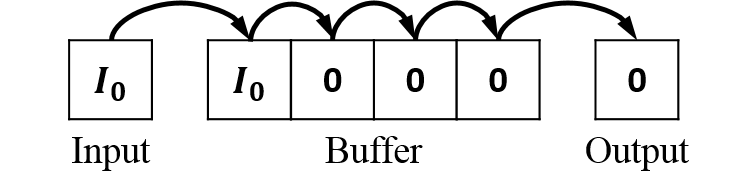
\includegraphics[width=\textwidth]{fig/buffer1.png}
        \caption{Primera Iteraci�n}
        \label{fig:buffer1}
    \end{subfigure}
    ~
    \begin{subfigure}[b]{0.3\textwidth}
    	\centering
        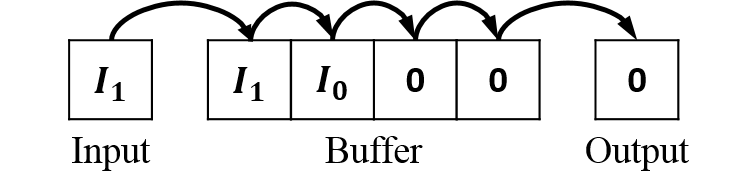
\includegraphics[width=\textwidth]{fig/buffer2.png}
        \caption{Segunda Iteraci�n}
        \label{fig:buffer2}
    \end{subfigure}
    ~ 
    \begin{subfigure}[b]{0.3\textwidth}
    	\centering
        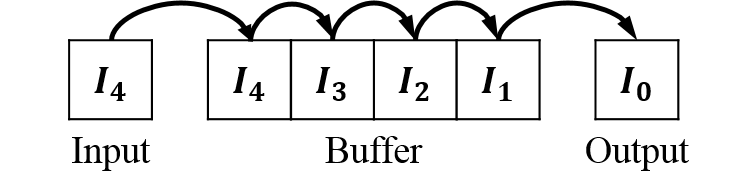
\includegraphics[width=\textwidth]{fig/buffer3.png}
        \caption{Quinta Iteraci�n}
        \label{fig:buffer3}
    \end{subfigure}
    \caption{\textbf{Funcionamiento del buffer de retardo. } Cada nodo dentro del substrato posee un buffer, con un largo dado por una red CPPN, que retardar� el flujo de informaci�n a trav�s de la red. En las im�genes se muestra un ejemplo de un nodo asignado con un buffer de tama�o 4, al que se le asignan por defecto todas sus casillas con valor cero. En la primera iteraci�n (a), la suma de todas las entradas al nodo es pasada por una funci�n de activaci�n previamente asignada dando como resultado el primer valor de entrada $\textit{I}_{0}$ al buffer, coloc�ndose al inicio de este y desplazando todos los dem�s valores contenidos en el buffer hacia la derecha. Luego el resultado de salida del nodo para la primera iteraci�n es el valor de la �ltima casilla del buffer antes del desplazamiento (cero). En la segunda iteraci�n (b), se entrega una nueva entrada $\textit{I}_{1}$ al buffer volviendo a desplazar cada valor contenido en el buffer hacia la derecha, obteni�ndose como salida el valor de la �ltima casilla del buffer antes del desplazamiento (cero aun). Al llegar a la quinta iteraci�n (c), se ingresa un nuevo valor a la entrada del buffer y se obtiene a la salida el valor $\textit{I}_{0}$ ingresado en la primera iteraci�n. }
    \label{fig:buffer}
\end{figure}

Cada nodo del substrato recibir� como entrada los valores de salida de cada uno de los dem�s nodos conectados a �l, multiplicados por sus respectivos pesos. Estos valores son sumados para posteriormente pasar el resultado por la funci�n de activaci�n del nodo e ingresar al inicio del buffer, desplazando los dem�s valores contenidos en �l hacia la derecha. El valor que queda fuera del buffer producto del desplazamiento se convierte en la salida final del nodo.

Todos estos retardos a lo largo de la red permitir�n incorporar variables temporales en la soluci�n del problema a solucionar, incorporando din�mica al sistema. Finalmente, el esquema b�sico del algoritmo del m�todo \(\tau\)-HyperNEAT se muestra a continuaci�n:

\begin{enumerate}
\item Elegir una configuraci�n de substrato, es decir, el posicionamiento de cada nodo, la asignaci�n de nodos de entrada y salida, y establecer un retardo m�ximo.
\item Inicializar una poblaci�n de redes CPPN con pesos asignados de forma aleatoria.
\item Repetir hasta encontrar una soluci�n:
	\begin{enumerate}
	\item Por cada miembro de la poblaci�n de redes CPPN:
		\begin{enumerate}[label=(\roman*)]
		\item Usar la red CPPN para determinar el factor de peso y el retardo de cada posible conexi�n en el substrato. Si el valor absoluto de la salida correspondiente al factor de peso de la red CPPN sobrepasa la magnitud de un umbral, se crea la conexi�n con el peso escalado apropiadamente y el porcentaje de retardo dado por la salida de la red CPPN.
		\item Se usa el substrato como una ANN en la tarea a resolver para determinar su desempe�o y asignar el resultado a la red CPPN.
		\end{enumerate}
	\item Reproducir las redes CPPN acorde al m�todo NEAT para producir una nueva poblaci�n de CPPNs correspondientes a una nueva generaci�n.
	\end{enumerate}
\end{enumerate}

Ya definidos el m�todo HyperNEAT y el m�todo propuesto \(\tau\)-HyperNEAT es posible realizar pruebas de desempe�o en la tarea de generaci�n de caminatas en robots con extremidades m�viles, pero para esto es necesario dise�ar una herramienta de comunicaci�n que permita al programa que usa alguno de estos m�todos de neuroevoluci�n comunicarse con el programa de simulaci�n en donde se ejecutar�n los entrenamientos de los robots en la generaci�n de caminatas. Adem\'as es necesario preparar el entorno de simulaci\'on y las plataformas rob�ticas que interactuar\'an dentro de esta. En el capitulo siguiente se mostrar� como realizar el dise�o de las plataformas rob�ticas a usar para la generaci�n de caminatas dentro del software de simulaci�n V-REP.



\chapter{ROBOTLIB: LIBRER�A PARA EL MANEJO DE ROBOTS REALES Y SIMULADOS}

RobotLib es una herramienta dise�ada para la comunicaci�n e interacci�n con entornos de simulaci�n y entornos reales de manera transparente y sencilla. RobotLib esta implementada en lenguaje C/C++ y funciona a modo de librer�a externa, entregando a disposici�n del usuario los recursos necesarios para poder obtener y entregar informaci�n a todos los entornos de trabajo (simulados o reales), inclusive de manera simultanea, de una forma simple y segura.

RobotLib esta compuesta por un conjunto de clases que se dividen en dos grupos, \textit{componentes} del entorno y \textit{controladores}. Los componentes del entorno son los objetos a manipular, como piezas, motores o sensores. Los controladores son objetos que permiten al usuario ejecutar acciones con los componentes del entorno, como por ejemplo posicionar piezas dentro de un entorno virtual, asignar posiciones a motores, o obtener lectura de sensores. As�, para que un usuario pueda manipular un componente de alg�n entorno de trabajo debe crear un objeto controlador para dicho entorno y un objeto correspondiente al tipo de componente, y adem�s, indicarle al objeto controlador el objeto componente que se desea manipular a trav�s de �l. Tambi�n es posible que un mismo componente sea controlado en distintos entornos de forma simultanea, creando tantos objetos controladores como sean necesarios para cada entorno, creando el objeto componente que se desea manipular, e indicarle a cada objeto controlador el componente a manipular. Esta �ltima estrategia es muy �til cuando se desea, por ejemplo, manipular un robot en un entorno virtual y en el entorno f�sico real de forma simultanea. A continuaci�n se explicar� de forma breve cada una de las clases fundamentales que componen RobotLib. Para obtener informaci�n m�s completa de esta librer�a debe revisarse el ap�ndice \textit{Implementaci�n de RobotLib}.

Los objetos controladores implementados son dos: el objeto \textit{RobotVREP} y \textit{USB2Dynamixel}. RobotVREP es el controlador implementado para manipular objetos dentro de software de simulaci�n VREP \cite{vrep}, el cual fue el software elegido para realizar los entrenamientos de generaci�n de caminatas en los robots con extremidades m�viles. USB2Dynamixel es el controlador implementado para controlar los motores de los robots a utilizar, los cuales son de la marca Dynamixel \cite{dyn}, a trav�s del dispositivo de comunicaci�n serial USB2Dynamixel dise�ado exclusivamente para dichos motores. 

Los objetos componentes implementados son tres: el objeto \textit{Object}, \textit{Joint} y \textit{CollisionObject}, en donde los �ltimos dos objetos heredan del primero. El objeto Object es la base de cualquier objeto existente en un experimento, y almacena un \textit{UniqueObjectId} asignado al objeto. El \textit{UniqueObjectId} es un n�mero �nico asignado a cada objeto al momento de ser creado, y permite que cada controlador pueda asociar dicho n�mero con el n�mero identificador interno respectivo de cada objeto, sin la necesidad de que un objeto deba almacenar tantos n�meros identificadores como controladores lo est�n controlando. En un programa de simulaci�n un Object puede representar, por ejemplo, un obst�culo dentro del escenario de simulaci�n, y usando las funciones disponibles en RobotVREP es posible obtener su posici�n, orientaci�n y velocidad, y asignarle una nueva posici�n y orientaci�n. En un entorno real un Object puede representar, por ejemplo, una IMU (del ingl�s \textit{Inertial Measurement Unit}), que con el procesamiento adecuado puede entregar, a trav�s del controlador respectivo, su posici�n, orientaci�n, velocidad y aceleraci�n. Para hacer uso de cualquier Object en alg�n entorno (simulado o real) solo debe indicarse al controlador respectivo que dicho Object estar� bajo su control, haciendo uso de la funci�n \textit{Controlador.addObject(Object *)} implementada en cada controlador \footnote{No esta implementado en el controlador USB2Dynamixel debido al no uso de sensores f�sicos.}, en donde el argumento entre par�ntesis corresponde al puntero del objeto a controlar. Funciones similares como \textit{addJoint(Joint *)} y \textit{addCollisionObject(CollisionObject *)} son usadas para trabajar con objetos Joint y CollisionObject respectivamente con el controlador RobotVREP; y addMotor(Joint *, int) con el controlador USB2Dynamixel, en donde el segundo argumento corresponde al ID del motor dynamixel f�sico. Una vez asignado el Object al controlador es posible, por ejemplo, obtener la posici�n de dicho objeto en coordenadas cartesianas dentro del entorno de simulaci�n (V-REP) usando la funci�n \textit{Controlador.getObjectPosition(Object *)}.

El objeto Joint es usado para representar cualquier tipo de motor que se desee utilizar, como un servomotor, un motor paso a paso, o uno de giro continuo. Si un Joint representa, por ejemplo, un servomotor de un brazo rob�tico, es posible asignarle una posici�n angular, o consultar cual es su posici�n actual para lograr mover el brazo. Si un Joint representa un motor de giro continuo, es posible variar su velocidad angular de giro, para por ejemplo, controlar un carro motorizado con ese tipo de motores. Cualquiera de dichas acciones debe realizarse usando las funciones disponibles en el controlador correspondiente, al cual previamente le fue asignado el control de dicho Joint con la funci�n \textit{addJoint(Joint *)}. De esta forma, a modo de ejemplo, si se desea asignar a un servomotor real una posici�n angular de $\pi$ radianes \footnote{por defecto el objeto Joint recibe y entrega valores en radianes, pero es posible elegir otro tipo de unidad disponible para evitar que el usuario deba realizar conversiones adicionales.}, se deben seguir los siguientes pasos:

\begin{itemize}
\item Informar al Joint la posici�n que necesita alcanzar, usando la funci�n \textit{setJointNextPosition((double)3.1415)}, en donde el argumento entre par�ntesis corresponde a la posici�n angular a adoptar de tipo doble flotante. Si se desea asignar una posici�n angular a m�s de un Joint se debe realizar esta misma operaci�n con cada uno de ellos.
\item Solicitar al controlador, que en este caso corresponde a un controlador USB2Dynamixel, que actualice la posici�n de cada uno de los motores usando la funci�n \textit{Controlador.move()}.
\end{itemize}

De esta forma, es posible mover todos los motores que se deseen de forma simultanea, como lo es en el caso de la generaci�n de caminatas en donde todas las extremidades de un robot deben moverse al mismo tiempo.

El objeto CollisionObject es usado para representar objetos que eventualmente puedan colisionar durante un experimento. En un entorno real un CollisionObject puede representar, por ejemplo, un sensor de tacto que al hacer contacto con otros objetos pueda indicar una posible colisi�n. En el software V-REP, un CollisionObject corresponde a una interacci�n entre dos entidades dentro del escenario que posean propiedades de colisi�n activas, pudiendo detectar si existe colisi�n entre estas. De esta forma, si por ejemplo se quisiera detectar una colisi�n entre el piso del escenario de simulaci�n y el torso de un robot, se deben seguir los siguientes pasos:

\begin{itemize}
\item Crear un objeto dentro del software de simulaci�n que relacione el par de entidades de posible colisi�n.
\item Crear un objeto CollisionObject correspondiente al objeto del punto anterior en el programa de entrenamiento.
\item Solicitar al controlador, que en este caso corresponde al controlador RobotVREP, que verifique si existe una colisi�n relacionada con el objeto del punto anterior usando la funci�n \textit{Controlador.readCollision(CollisionObject *)}, en donde el argumento entre par�ntesis corresponde al puntero del objeto que relaciona el par de entidades a colisionar. Esta funci�n retornar� un valor booleano verdadero si existe una colisi�n entre el par de entidades, o falso si no existe colisi�n.
\end{itemize}

Con el uso de los objetos mencionados anteriormente es posible efectuar cualquier tipo de experimento relacionado con rob�tica m�vil, por lo que RobotLib es una herramienta indispensable para el estudio de la rob�tica para cualquier rama de investigaci�n. A continuaci�n se muestra un programa de prueba, escrito en C/C++, en donde se acelera un motor de giro continuo unido a una h�lice sobre la cual hay un cilindro (figura \ref{prueba}) que es expulsado por efecto de la aceleraci�n centr�fuga.

\begin{figure}[t]
\centering
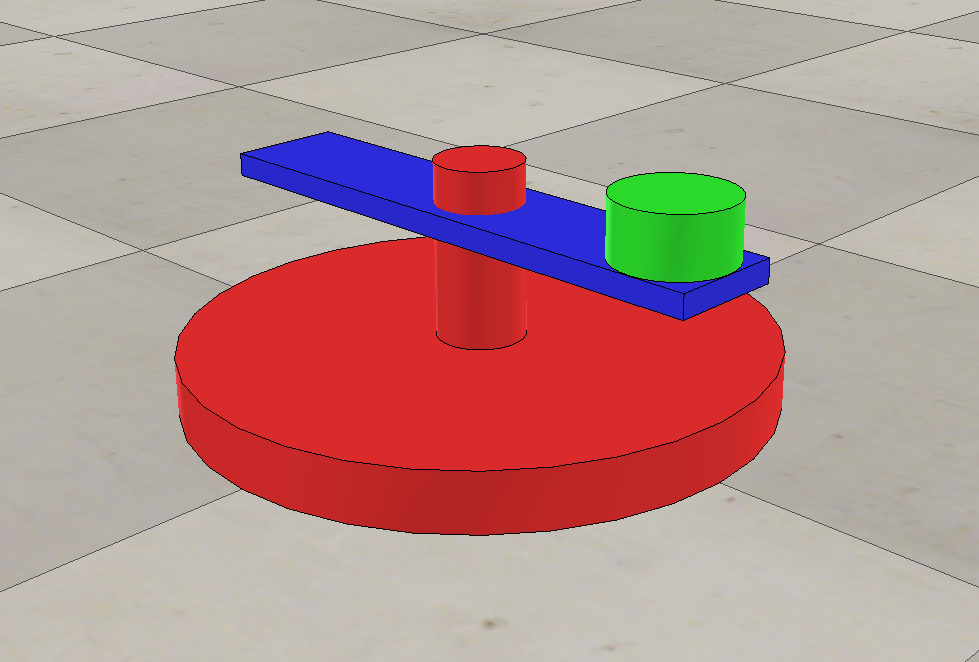
\includegraphics[width=0.8\textwidth]{fig/prueba.png}
\caption{\textbf{Escenario de prueba de la librer�a RobotLib. }El escenario de simulaci�n de la figura muestra una h�lice azul montada en una base que gira con el uso de un motor o \textit{Joint}, y un cilindro verde sobre un extremo de la h�lice. El experimento, realizado como ejemplo de uso de la librer�a RobotLib, tiene como objetivo hacer girar la h�lice y acelerarla hasta expulsar el cilindro de sobre ella producto de la fuerza centrifuga generada sobre el cilindro producto del giro.}
\label{prueba_robotlib}
\end{figure}

\lstset{language=C++,
		frame=L,
		basicstyle=\footnotesize, 
		identifierstyle=\color{black},
		keywordstyle=\bfseries\color{green!40!black},
		stringstyle=\color{red!85!white},
		commentstyle=\color{cyan!70!black},
		morecomment=[l][\color{blue!70!white}]{\#},		
		showstringspaces=false,
		tabsize=2,
		numbers=left,
		lineskip={-1.5pt},
		breaklines=true
}

\newpage

\lstinputlisting{code/example_vrep.cpp}

Como se aprecia en la linea 4 del c�digo anterior, una vez instalada la librer�a RobotLib, es posible utilizarla solo incluy�ndola como all� se muestra. El programa crea un objeto RobotVREP para controlar los objetos dentro del software V-REP, un objeto Joint para el motor que hace girar la h�lice, y un objeto CollisionObject que relaciona el contacto entre la h�lice y el cilindro, y a�ade estos dos �ltimos al controlador. Luego, se inicia una simulaci�n, y se aumenta la velocidad de giro del Joint hasta que se detectan dos ``no colisiones''\footnote{Por posibles inexactitudes de la escena y los objetos dentro de ella se producen breves detecciones de no colisi�n entre objetos que si est�n colisionando, por lo que se verifican dos no colisiones consecutivas para asegurar que los objetos no est�n colisionando realmente.} consecutivas relacionadas con el CollisionObject, producto de la ca�da del cilindro desde la superficie de la h�lice. Una vez confirmada la ca�da del cilindro de la superficie de la h�lice se reduce la velocidad del Joint hasta detenerlo para finalmente detener la simulaci�n. En el capitulo siguiente se mostrar� como realizar el dise�o de las plataformas rob�ticas a usar para la generaci�n de caminatas dentro del software de simulaci�n V-REP.




RobotLib\footnote{\url{https://github.com/osilvam/RobotLib}} es una herramienta dise�ada en el marco de esta memoria\footnote{La librer�a RobotLib fue dise�ada en conjunto con el estudiante de Ingenier�a Civil Electr�nica Pascal Sigel Olivares} para la comunicaci�n e interacci�n con entornos de simulaci�n y entornos reales de manera transparente y sencilla. RobotLib esta implementada en lenguaje C/C++ y funciona a modo de librer�a externa, entregando a disposici�n del usuario los recursos necesarios para poder obtener y entregar informaci�n a todos los entornos de trabajo (simulados o reales), inclusive de manera simultanea, de una forma simple y segura.

RobotLib esta compuesta por un conjunto de clases que se dividen en dos grupos, \textit{componentes} del entorno y \textit{controladores}. Los componentes del entorno son los objetos a manipular, como piezas, motores o sensores. Los controladores son clases que permiten al usuario ejecutar acciones con los componentes del entorno, como por ejemplo posicionar piezas dentro de un entorno virtual, asignar posiciones a motores, u obtener lectura de sensores. As�, para que un usuario pueda manipular un componente de alg�n entorno de trabajo debe instanciar un objeto de la clase controlador para dicho entorno y un objeto de la clase correspondiente al tipo de componente, y adem�s, indicarle al objeto controlador el objeto componente que se desea manipular a trav�s de �l. Tambi�n es posible que un mismo componente sea controlado en distintos entornos de forma simultanea, instanciando tantos objetos controladores como sean necesarios para cada entorno, instanciando el objeto componente que se desea manipular, e indicarle a cada objeto controlador el componente a manipular. Esta �ltima estrategia es muy �til cuando se desea, por ejemplo, manipular un robot en un entorno virtual y en el entorno f�sico real de forma simultanea. A continuaci�n se explicar� de forma breve cada una de las clases fundamentales que componen RobotLib.

Las clases controladores implementadas son dos:

\begin{itemize}
\item \textbf{RobotVREP }  RobotVREP es el controlador implementado para manipular objetos dentro de software de simulaci�n VREP \cite{vrep}, el cual fue el software elegido para realizar los entrenamientos de generaci�n de caminatas en los robots con extremidades m�viles.

\item \textbf{USB2Dynamixel } USB2Dynamixel es el controlador implementado para controlar los motores de los robots a utilizar, los cuales son de la marca Dynamixel \cite{dyn}, a trav�s del dispositivo de comunicaci�n serial USB2Dynamixel dise�ado exclusivamente para dichos motores. 
\end{itemize}

Las clases componentes implementadas son tres:

\begin{itemize}
\item \textbf{Object } La clase Object es la base de cualquier objeto existente en un experimento, y almacena un \textit{UniqueObjectId} asignado al objeto. El \textit{UniqueObjectId} es un n�mero �nico asignado a cada objeto al momento de ser creado, y permite que cada controlador pueda asociar dicho n�mero con el n�mero identificador interno respectivo de cada objeto, sin la necesidad de que un objeto deba almacenar tantos n�meros identificadores como controladores lo est�n controlando. En un programa de simulaci�n un Object puede representar, por ejemplo, un obst�culo dentro del escenario de simulaci�n, y usando las funciones disponibles en RobotVREP es posible obtener su posici�n, orientaci�n y velocidad, y asignarle nuevos valores a estas variables. En un entorno real un Object puede representar, por ejemplo, una IMU (del ingl�s \textit{Inertial Measurement Unit}), que con el procesamiento adecuado puede entregar, a trav�s del controlador respectivo, su posici�n, orientaci�n, velocidad y aceleraci�n. Para hacer uso de cualquier Object en alg�n entorno (simulado o real) solo debe indicarse al controlador respectivo que dicho Object estar� bajo su control, haciendo uso de la funci�n \texttt{Controlador.addObject(Object *)} implementada en cada controlador \footnote{No esta implementado en el controlador USB2Dynamixel debido al no uso de sensores f�sicos.}, en donde el argumento entre par�ntesis corresponde al puntero del objeto a controlar. Funciones similares como \texttt{addJoint(Joint *)} y \texttt{addCollisionObject(CollisionObject *)} son usadas para trabajar con objetos Joint y CollisionObject respectivamente con el controlador RobotVREP; y addMotor(Joint *, int) con el controlador USB2Dynamixel, en donde el segundo argumento corresponde al ID del motor dynamixel f�sico. Una vez asignado el Object al controlador es posible, por ejemplo, obtener la posici�n de dicho objeto en coordenadas cartesianas dentro del entorno de simulaci�n (V-REP) usando la funci�n \texttt{Controlador.getObjectPosition(Object *)}.

\item \textbf{Joint} La clase Joint, que hereda de la clase Object, es usado para representar cualquier tipo de motor que se desee utilizar, como un servomotor, un motor paso a paso, o uno de giro continuo. Si un Joint representa, por ejemplo, un servomotor de un brazo rob�tico, es posible asignarle una posici�n angular, o consultar cual es su posici�n actual para lograr mover el brazo. Si un Joint representa un motor de giro continuo, es posible variar su velocidad angular de giro, para por ejemplo, controlar un carro motorizado con ese tipo de motores. Cualquiera de dichas acciones debe realizarse usando las funciones disponibles en el controlador correspondiente, al cual previamente le fue asignado el control de dicho Joint con la funci�n \texttt{addJoint(Joint *)}. De esta forma, a modo de ejemplo, si se desea asignar a un servomotor real una posici�n angular de $\pi$ radianes \footnote{por defecto el objeto Joint recibe y entrega valores en radianes, pero es posible elegir otro tipo de unidad disponible para evitar que el usuario deba realizar conversiones adicionales.}, se deben seguir los siguientes pasos:
\begin{enumerate}
\item Informar al Joint la posici�n que necesita alcanzar, usando la funci�n \texttt{setJointNextPosition((double)3.1415)}, en donde el argumento entre par�ntesis corresponde a la posici�n angular a adoptar de tipo doble flotante. Si se desea asignar una posici�n angular a m�s de un Joint se debe realizar esta misma operaci�n con cada uno de ellos.

\item Solicitar al controlador, que en este caso corresponde a un controlador USB2Dynamixel, que actualice la posici�n de cada uno de los motores usando la funci�n \texttt{Controlador.move()}.
\end{enumerate}

De esta forma, es posible mover todos los motores que se deseen de forma simult�nea, como lo es en el caso de la generaci�n de caminatas en donde todas las extremidades de un robot deben moverse al mismo tiempo.

\item \textbf{CollisionObject } La clase CollisionObject es usada para representar objetos que eventualmente puedan colisionar durante un experimento. En un entorno real un CollisionObject puede representar, por ejemplo, un sensor de tacto que al hacer contacto con otros objetos pueda indicar una posible colisi�n. En el software V-REP, un CollisionObject corresponde a una interacci�n entre dos entidades dentro del escenario que posean propiedades de colisi�n activas, pudiendo detectar si existe colisi�n entre estas. De esta forma, si por ejemplo se quisiera detectar una colisi�n entre el piso del escenario de simulaci�n y el torso de un robot, se deben seguir los siguientes pasos:

\begin{enumerate}
\item Crear un objeto dentro del software de simulaci�n que relacione el par de entidades de posible colisi�n.

\item Instanciar un objeto CollisionObject correspondiente al objeto del punto anterior en el programa de entrenamiento.

\item Solicitar al controlador, que en este caso corresponde al controlador RobotVREP, que verifique si existe una colisi�n relacionada con el objeto del punto anterior usando la funci�n \texttt{Controlador.readCollision\-(CollisionObject *)}, en donde el argumento entre par�ntesis corresponde al puntero del objeto que relaciona el par de entidades a colisionar. Esta funci�n retornar� un valor booleano verdadero si existe una colisi�n entre el par de entidades, o falso si no existe colisi�n.
\end{enumerate}

\end{itemize}

Con el uso de las clases mencionadas anteriormente es posible efectuar cualquier tipo de experimento relacionado con rob�tica m�vil, por lo que RobotLib es una herramienta indispensable para el estudio de la rob�tica para cualquier rama de investigaci�n. A continuaci�n se muestra un programa de prueba, escrito en C/C++, en donde se acelera un motor de giro continuo unido a una h�lice sobre la cual hay un cilindro (figura \ref{prueba_robotlib}) que es expulsado por efecto de la aceleraci�n centr�fuga.

\lstset{language=C++,
		frame=L,
		basicstyle=\footnotesize, 
		identifierstyle=\color{black},
		keywordstyle=\bfseries\color{green!40!black},
		stringstyle=\color{red!85!white},
		commentstyle=\color{cyan!70!black},
		morecomment=[l][\color{blue!70!white}]{\#},		
		showstringspaces=false,
		tabsize=2,
		numbers=left,
		lineskip={-1.5pt},
		breaklines=true
}

\newpage

\lstinputlisting{code/example_vrep.cpp}

Como se aprecia en la linea 2 del c�digo anterior, una vez instalada la librer�a RobotLib, es posible utilizarla solo incluy�ndola como all� se muestra. El programa crea un objeto RobotVREP para controlar los objetos dentro del software V-REP, un objeto Joint para el motor que hace girar la h�lice, y un objeto CollisionObject que relaciona el contacto entre la h�lice y el cilindro, y a�ade estos dos �ltimos al controlador. Luego, se inicia una simulaci�n, y se aumenta la velocidad de giro del Joint hasta que se detectan dos ``no colisiones''\footnote{Por posibles inexactitudes de la escena y los objetos dentro de ella se producen breves detecciones de no colisi�n entre objetos que si est�n colisionando, por lo que se verifican dos no colisiones consecutivas para asegurar que los objetos no est�n colisionando realmente.} consecutivas relacionadas con el CollisionObject, producto de la ca�da del cilindro desde la superficie de la h�lice. Una vez confirmada la ca�da del cilindro de la superficie de la h�lice se reduce la velocidad del Joint hasta detenerlo para finalmente detener la simulaci�n. Toda la informaci�n necesaria para el manejo de la librer�a RobotLib puede ser obtenida a trav�s de su documentaci�n en \textit{Doxygen} generada por medio del mismo makefile de instalaci�n de la librer�a. 

Finalmente es posible iniciar los entrenamientos para generar las caminatas en los robots, lo cual ser� relatado en el siguiente cap�tulo.

\begin{figure}[t]
\centering
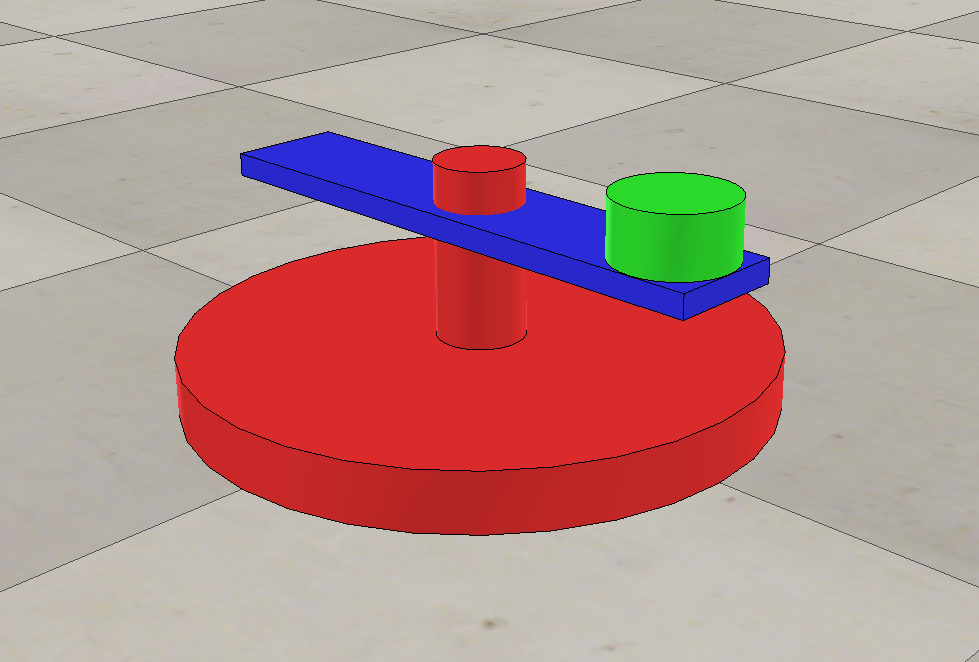
\includegraphics[width=0.8\textwidth]{fig/prueba.png}
\caption{\textbf{Escenario de prueba de la librer�a RobotLib. }El escenario de simulaci�n de la figura muestra una h�lice azul montada en una base que gira con el uso de un motor o \textit{Joint}, y un cilindro verde sobre un extremo de la h�lice. El experimento, realizado como ejemplo de uso de la librer�a RobotLib, tiene como objetivo hacer girar la h�lice y acelerarla hasta expulsar el cilindro de sobre ella producto de la fuerza centrifuga generada sobre el cilindro producto del giro.}
\label{prueba_robotlib}
\end{figure}






\chapter{SIMULACI�N DE CAMINATAS}

Con el fin de lograr que las plataformas rob�ticas aprendan a mover sus extremidades de tal manera de generar una caminata que le permita desplazarse es necesario que estas entrenen. Un entrenamiento consiste en un gran n�mero de simulaciones en donde un robot intentar� realizar movimientos con el objetivo de desplazarse. Cada simulaci�n tendr� una duraci�n m�xima de 6 segundos durante los cuales el robot podr� moverse, midi�ndose su desempe�o una vez finalizada la simulaci�n. Durante el trascurso de los 6 segundos de simulaci�n el programa de entrenamiento comprobar� iteraci�n tras iteraci�n la existencia de colisiones entre las piezas de la estructura del robot y el suelo del escenario de simulaci�n (exceptuando las puntas de las patas que deben hacer contacto con el suelo para lograr el desplazamiento del robot). Si una colisi�n es detectada, la simulaci�n es terminada de forma abrupta, y los resultados de dicha simulaci�n no son contemplados para el entrenamiento.

Para el caso de HyperNEAT y \(\tau\)-HyperNEAT cada simulaci�n de 6 segundo busca verificar el desempe�o en la generaci�n de caminatas de ambos m�todos. Para ambos casos se ha establecido una configuraci�n de substrato del tipo state-space sandwich, con una capa de entrada, una capa de salida y solo una capa oculta o intermedia. A la capa de entrada del substrato ingresar�n los valores de las �ltimas posiciones de los motores de cada robot, junto a dos se�ales senoidales desfasadas en 90 grados; as� si el robot posee 12 motores para mover sus extremidades, la capa de entrada poseer� 14 nodos. A la capa intermedia, conformada por $n^{2}$ nodos con $n$ como el n�mero de patas del robot, ingresar�n las se�ales provenientes de la capa de entrada. Finalmente la capa de salida, conformada por tantos nodos como motores tenga el robot a utilizar, recibir� las se�ales provenientes de los nodos de la capa intermedia, y sus salidas corresponder�n a las nuevas posiciones que deben adoptar los motores del robot. Para el c�lculo de una nueva iteraci�n (nuevas posiciones para los motores), las posiciones de los motores obtenidas anteriormente a la salida del substrato ser�n las nuevas entradas de este. De esta forma el substrato en ambos m�todos tendr� la labor de generar las se�ales de accionamiento de cada motor para lograr el desplazamiento del robot, a partir de las dos se�ales senoidales adicionales de entrada.

Para el caso de HyperNEAT, la red CPPN que establece las conexiones en el substrato posee sus cuatro entradas b�sicas de coordenadas $x$ e $y$ de los nodos de origen y destino, adem�s de dos entradas adicionales de informaci�n referente al espaciamiento entre ellos a lo largo de los ejes cartesianos, y como salida los pesos de las conexiones entre nodos de la capa de entrada e intermedia y entre la capa intermedia y de salida. Para el caso de \(\tau\)-HyperNEAT, la red CPPN que establece las conexiones en el substrato posee las mismas entradas que para el caso de HyperNEAT, pero como salida, adem�s de entregar los pesos de las conexiones entre nodos de la capa de entrada e intermedia y entre la capa intermedia y de salida entrega los retardos correspondientes a dichas conexiones. En la figura \ref{fig:h_tauh_structure} se puede apreciar un ejemplo de configuraci�n de ambos m�todos para el caso de un robot cuadr�pedo de tres grados de libertad por extremidad.

\begin{figure}[ht!]
	\centering
	\begin{subfigure}[b]{0.71\textwidth}
		\centering
        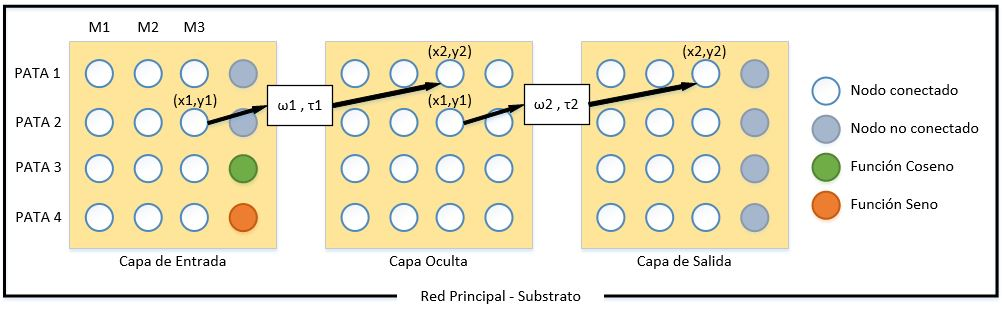
\includegraphics[width=\textwidth]{fig/hsubstrate.JPG}
        \label{fig:hsubstrate}
    \end{subfigure}
    ~
    \begin{subfigure}[b]{0.255\textwidth}
    	\centering
        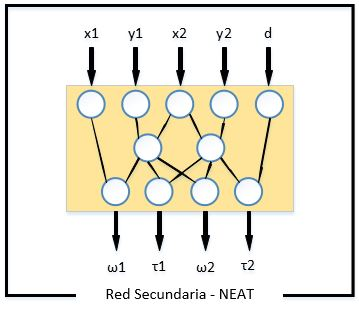
\includegraphics[width=\textwidth]{fig/hcppn.JPG}
        \label{fig:hcppn}
    \end{subfigure}
    
    \centering
	\begin{subfigure}[b]{0.71\textwidth}
		\centering
        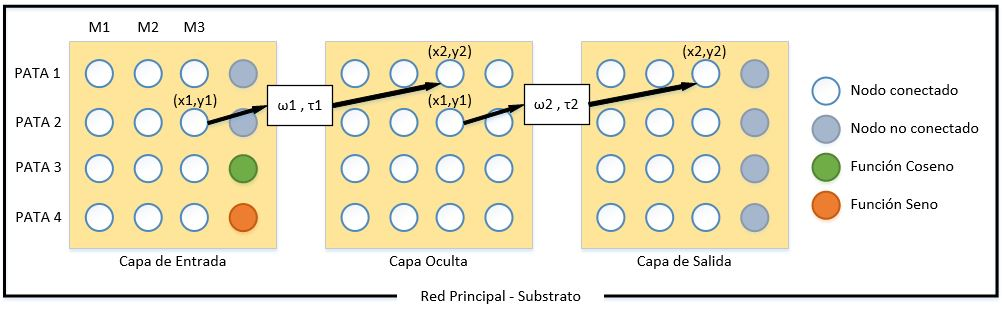
\includegraphics[width=\textwidth]{fig/tauhsubstrate.JPG}
        \label{fig:tauhsubstrate}
    \end{subfigure}
    ~
    \begin{subfigure}[b]{0.255\textwidth}
    	\centering
        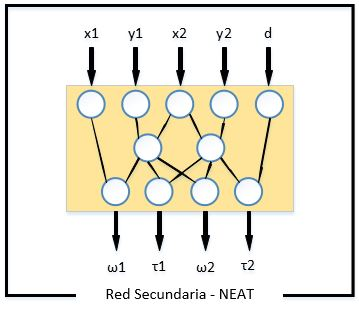
\includegraphics[width=\textwidth]{fig/tauhcppn.JPG}
        \label{fig:tauhcppn}
    \end{subfigure}
    \caption{\textbf{Esquema estructural de HyperNEAT y \(\tau\)-HyperNEAT.} En la figura, los recuadros superiores e inferiores muestran el esquema estructural del m�todo HyperNEAT y \(\tau\)-HyperNEAT respectivamente, usado en los experimentos con un robot cuadr�pedo de 3 grados de libertad por extremidad. Ambos recuadros derechos corresponden a la estructura del substrato del m�todo respectivo, mientras que los recuadros izquierdos corresponden a la estructura b�sica de la red CPPN, en las que es posible apreciar la diferencia en la cantidad de salidas entre ambas debido a que en \(\tau\)-HyperNEAT la red CPPN debe calcular los retardos de las conexiones en el substrato, adem�s de los pesos correspondientes a ellas.}
    \label{fig:h_tauh_structure}
\end{figure}

Una vez finalizada una simulaci�n exitosa (no se detectaron colisiones), es necesario medir y evaluar el desempe�o de la caminata generada por e robot. La determinaci�n de que tan bueno o que tan malo fue el desempe�o del robot durante una simulaci�n es un aspecto cr�tico del entrenamiento, ya que esto determinar� de que manera evolucionar�n las CPPNs encargadas de generar las conexiones en el substrato de HyperNEAT y \(\tau\)-HyperNEAT. En la siguiente secci�n se ahondar� respecto a la medici�n y evaluaci�n del desempe�o de las caminatas generadas por ambos m�todos.

\section{FUNCIONES DE DESEMPE�O}

Con el objetivo de lograr medir correctamente el desempe�o de las caminatas de cada robot es que se observar�n dos variables importantes en cada simulaci�n, la frecuencia de oscilaci�n de cada uno de los motores y la m�xima distancia alcanzada por el robot. Ambas variables son medidas los �ltimos cinco segundos de simulaci�n, debido a que es posible que ocurran acciones no deseadas del robot inmediatamente al inicio de cada simulaci�n, evit�ndose as� lecturas err�neas de dichas variables. 

La frecuencia de cada motor es calculada observando los cambios en el signo de la pendiente en el movimiento de este entre una iteraci�n y otra, siendo un cambio de signo entre iteraciones consecutivas un cambio en la direcci�n en que se mueve el motor. As� dos cambios de direcci�n en el movimiento de un motor indicar�n el suceso de un periodo completo de se�al de dicho motor. Una vez obtenida la frecuencia de cada uno de los motores se promedian las frecuencias correspondientes a motores de la misma extremidad y dicho promedio es ingresado a la funci�n del c�lculo del desempe�o de la caminata seg�n la frecuencia, mostrada en la figura \ref{fig:fitnessfrec}. Por �ltimo el desempe�o final correspondiente a la frecuencia estar� dado por el promedio de las salidas de la funci�n de desempe�o de frecuencias de cada extremidad.

\begin{figure}[ht!]
	\centering
	\begin{subfigure}[b]{0.48\textwidth}
		\centering
        
\includegraphics[width=\textwidth]{fig/usmLogo.png}
        \caption{Funci�n de desempe�o de la frecuencia.}
        \label{fig:fitnessfrec}
    \end{subfigure}
    ~
    \begin{subfigure}[b]{0.48\textwidth}
    	\centering
        
\includegraphics[width=\textwidth]{fig/usmLogo.png}
        \caption{Funci�n de desempe�o de la distancia.}
        \label{fig:fitnessdist}
    \end{subfigure}
    \caption{\textbf{Funciones de desempe�o del entrenamiento.} En esta figura se muestran las funciones de desempe�o usadas para calificar que tan exitosa fue una caminata en el entrenamiento.}
    \label{fig:fitness}
\end{figure}

La distancia final alcanzada por el robot durante la simulaci�n es calculada por la diferencia de distancia entre el punto donde se posiciona el robot en el segundo uno de simulaci�n y el punto final que alcanza. Luego dicha distancia es ingresada a la funci�n del c�lculo del desempe�o de la caminata seg�n la distancia alcanzada, mostrada en la figura \ref{fig:fitnessdist}.

El resultado final del desempe�o de la caminata de un robot durante una simulaci�n estar� dado por una funci�n multi-objetivo compuesta por las dos funciones mostradas anteriormente, en donde prevalecer� el menor resultado entre ellas con el fin de evolucionar las CPPNs forzando a mejorar siempre el resultado de la variable con m�s problemas. As� si el desempe�o de la frecuencia y la distancia, por ejemplo, da como resultado 6 y 4 respectivamente, el desempe�o final del robot ser� de 4. Finalmente, el resultado obtenido ser� asignado a la red CPPN usada en la respectiva simulaci�n. Una vez comprendido el funcionamiento de cada simulaci�n y el c�lculo del desempe�o en cada una de estas es posible entender la estructura b�sica de un entrenamiento, como se muestra en la siguiente secci�n.

\section{ESTRUCTURA B�SICA DE UN ENTRENAMIENTO}

Un entrenamiento comienza con una poblaci�n o grupo inicial de CPPNs, cuyo n�mero es indicado por el usuario con anterioridad, conformando la primera generaci�n de redes a entrenar. Cada una de estas redes crear� un patr�n de conectividad en el substrato de HyperNEAT y \(\tau\)-HyperNEAT y se probar� en una simulaci�n para medir su desempe�o. Una vez que se midieron y evaluaron todas las CPPNs de la primera generaci�n deber�n evolucionar en una nueva generaci�n de redes CPPN, a trav�s del m�todo NEAT usado en ambos m�todos, del mismo tama�o de la poblaci�n inicial. Las CPPNs que conforman esta nueva generaci�n deber�n ser nuevamente probadas y evaluadas seg�n su desempe�o para dar origen a la generaci�n siguiente. Esto debe realizarse tantas veces como generaciones haya establecido el usuario para el entrenamiento dado. De esta forma si el usuario, por ejemplo, defini� al inicio del entrenamiento un n�mero de 100 generaciones con una poblaci�n de 100 CPPNs por generaci�n, el entrenamiento finalizar� una vez probadas las 10 mil CPPNs que conforman la totalidad de las generaciones. El proceso descrito anteriormente es la base de todo entrenamiento usando los m�todos HyperNEAT y \(\tau\)-HyperNEAT para cualquier experimento dado. En la secci�n siguiente se ahondar� en el funcionamiento del programa de entrenamiento, escrito en lenguaje C/C++, que hace uso de las herramientas presentadas anteriormente para generar caminatas en robots con extremidades m�viles.

\section{PROGRAMA DE ENTRENAMIENTO}

Una de las grandes problem�ticas presentes en los entrenamientos que comprometen periodos de tiempo real para su ejecuci�n es la extensa duraci�n de estos. El entrenamiento para la generaci�n de caminatas en robots con extremidades m�viles es uno de estos, ya que cada una de las simulaciones del entrenamiento debe durar los 6 segundos definidos para esta. As�, si un entrenamiento esta estipulado para evolucionar una poblaci�n de 100 CPPNs durante 100 generaciones, el tiempo estimado para su realizaci�n sobrepasa las 16 horas.

Debido a esta raz�n es que el programa de entrenamiento tiene la posibilidad de usar hebras (thread en ingles) para acelerar su ejecuci�n. El uso de hebras permitir� disminuir el tiempo total usado para el entrenamiento, ya que de esta forma ser� posible utilizar simult�neamente tantos simuladores como hebras corra el programa \footnote{Si bien una computadora actual puede ejecutar una gran cantidad de hebras simult�neamente, no podr� ejecutar la misma cantidad de simuladores debido a que la demanda de recursos generada por estos es elevada.}. De esta forma si el usuario, por ejemplo, indica el uso de 2 hebras, la poblaci�n de cada generaci�n ser� dividida en 2, ejecutando cada grupo de CPPNs en un simulador distinto y dividiendo el tiempo de entrenamiento a la mitad.

Una vez iniciado el programa de entrenamiento, este crear� todos los objetos necesarios para controlar al robot a usar dentro del simulador, usando la ya mencionada librer�a RobotLib. De usar m�s de un simulador, se deber�n crear tantos objetos repetidos como simuladores se ejecuten. Tambi�n se deben crear los objetos correspondientes al m�todo a utilizar (HyperNEAT o \(\tau\)-HyperNEAT), que al igual que en el caso de RobotLib, deben corresponder en n�mero a la cantidad de simuladores o hebras estipuladas para el entrenamiento.

Ya creadas todas las entidades necesarias para el funcionamiento de los m�todos de neuroevoluci�n y de los simuladores el programa continuar� con un bucle for que iterar� tantas veces como generaciones se hayan estipulado para el entrenamiento, y en cada ciclo de este se iniciar�n las hebras que se dividir�n la poblaci�n de CPPNs para ejecutar las simulaciones correspondientes a cada una de ellas. Luego que cada una de las hebras termine de probar y evaluar cada unas de las CPPNs asignadas, estas terminar�n su ejecuci�n volviendo el programa al bucle for para posteriormente evolucionar la poblaci�n de CPPNs en una nueva generaci�n y completar nuevamente un nuevo ciclo del bucle. Una vez realizados todos los ciclos del bucle for se obtendr� la red CPPN capaz de crear el patr�n de conectividad m�s adecuado sobre el substrato del m�todo usado, logrando la caminata con el mejor desempe�o del entrenamiento.

Para comprobar el funcionamiento de HyperNEAT y \(\tau\)-HyperNEAT en la generaci�n de caminatas en robots con extremidades m�viles se entrenar�n a 3 robots distintos: Quadratot, ArgoV2 y Rosita (ver Figura \ref{robots}), siendo el primero un robot dise�ado por el Investigador de la Universidad de Chile Juan Crist�bal Zagal, con el objeto de ser usado para comprobar el funcionamiento de distintos m�todos para la generaci�n de caminatas; y los �ltimos dos, robots dise�ados por el estudiante de Ingenier�a en Dise�o de Productos Cristian Osorio M�ndez para el Departamento de Electr�nica de La Universidad T�cnica Federico Santa Mar�a. En la secci�n siguiente se mostrar�n los resultados de los entrenamientos realizados sobre cada uno de estos robots usando ambos m�todos de neuroevoluci�n. Todos los c�digos utilizados en la siguiente secci�n pueden ser descargados desde el repositorio Github \url{https://github.com/osilvam/Memoria} y probados de manera f�cil y sencilla.

\section{RESULTADOS DE LOS ENTRENAMIENTOS}

Tal como se mencion� anteriormente, los entrenamientos para la generaci�n de caminatas usando los m�todos de neuroevoluci�n HyperNEAT y \(\tau\)-HyperNEAT se aplicar�n en 3 plataformas rob�ticas, Quadratot, ArgoV2 y Rosita. A continuaci�n se mostrar�n los resultados obtenidos para cada una de ellas.

\subsection{QUADRATOT}

\begin{itemize}
\item[\textbf{HyperNEAT}] jkwnajkw
\item[\textbf{\(\tau\)-HyperNEAT}] jkwnajkw
\end{itemize}



\section{DISCUSION Y COMPARACION DE LOS RESULTADOS OBTENIDOS}

En este trabajo de memoria se ha implementado un nuevo m�todo de neuroevoluci�n, llamado \(\tau\)-HyperNEAT, con el objetivo de ponerlo a prueba en la tarde de generaci�n de caminatas en robots con extremidades m�viles. En particular, se ha planteado la hip�tesis de que este nuevo m�todo de neuroevoluci�n, al incorporar retardos de tiempo en las conexiones a lo largo de la red principal, tendr� mejoras en su desempe�o final y generar� caminatas con caracter�sticas cualitativas superiores.

Luego de analizar todos los resultados obtenidos a partir de los experimentos realizados es posible concluir lo siguiente.

\begin{enumerate}
\item En la tarea de generaci�n de caminatas, no hubo diferencias cuantitativas en los resultados obtenidos a trav�s de los m�todos HyperNEAT y \(\tau\)-HyperNEAT, obteni�ndose en ambos casos el mismo desempe�o de a cuerdo a las variables involucradas en el proceso de calificaci�n de las caminatas.
\item En la tarea de generaci�n de caminatas, \(\tau\)-HyperNEAT logr� desarrollar, casi en un 100\%, caminatas con movimientos arm�nicos y coordinados, similares a comportamientos vistos en la naturaleza. Esto pudo ser observado en los gr�ficos de las se�ales de los motores generadas por \(\tau\)-HyperNEAT, evidenciandose las diferencias y similitudes de fases vistas entre distintas extremidades y motores de una misma extremidad respectivamente.
\end{enumerate}

Ya que las capacidades de HyperNEAT para generar caminatas con movimientos arm�nicos y coordinados fueron pr�cticamente nulas frente a las capacidades mostradas por el m�todo \(\tau\)-HyperNEAT, es posible afirmar que este nuevo m�todo, al incorporar retardos de tiempo a lo largo de su red principal, logra afrontar y resolver de mejor manera problemas din�micos que involucran variables temporales, como lo es en particular, la generaci�n de caminatas en robots con extremidades m�viles.

\section{TRABAJO FUTURO}

Dados los resultados obtenidos en este trabajo de memoria, se considera que los siguientes
son temas para trabajo futuro, enfocados tanto en la generaci�n de caminatas como en la de cualquier tipo de experimento en donde se puedan aprovechar las capacidades de las redes HyperNEAT y \(\tau\)-HyperNEAT.

\begin{itemize}
\item Verificar las posibles variaciones en el desempe�o del m�todo \(\tau\)-HyperNEAT para distintos valores del retardo m�ximo ($\tau_{max}$) en las conexiones de la red.
\item Experimentar con diferentes configuraciones geom�tricas en el substrato de las redes HyperNEAT y \(\tau\)-HyperNEAT, con el objetivo de explotar al m�ximo las capacidades de ambas redes.
\item Formular y probar nuevas funciones de desempe�o para lograr clasificar de manera �ptima la correcta ejecuci�n de una caminata, favoreciendo siempre el proceso de evoluci�n de caminatas realmente efectivas y as� obtener mejores resultados.
\item Traspasar los resultados obtenidos en simulaciones a un entorno real, emulando de manera correcta las din�micas presentes en cada robot.
\end{itemize}

\renewcommand{\refname}{Referencias}
\begin{thebibliography}{99}

\bibitem{hyperneat} STANLEY, K.O., D'AMBROSIO, D., and GAUSI, J. (2009). ``A hypercube-based encoding for evolving large-scale neural networks''. Artificial Life, 15(2):185-212.

\bibitem{neat} STANLEY, K.O., and MIIKKULAINEN, R. (2002). ``Evolving neural networks through augmenting topologies''. Evolutionary Computation, 10(2):99-127.

\bibitem{zykov} ZYKOV, V., BONGARD, J., and LIPSON, H. (2004). ``Evolving Dynamic Gaits on a Physical Robot'', Proceedings of Genetic and Evolutionary Computation Conference, Late Breaking Paper, GECCO.

\bibitem{hornby} HORNBY, G.S., TAKAMURA, S., YAMAMOTO, T., and FUJITA M. (2005). ``Autonomous Evolution of Dynamic Gaits with Two Quadruped Robots''.

\bibitem{clune} CLUNE, J., BECKMAN, B.E., OFRIA, C., and PENNOCK, R.T. (2009). ``Evolving coordinated quadruped gaits with the HyperNEAT generative encoding'', In Proceedings of the IEEE Congress on Evolutionary Computing.

\bibitem{yosinski} YOSINSKI, J., CLUNE, J., HIDALGO, D., NGUYEN, S., ZAGAL, J.C., and LIPSON, H. (2011). ``Evolving robot gaits in hardware: the HyperNEAT generative encoding vs. parameter optimization'', In Proceedings of the 20th European Conference on Artificial Life.

\bibitem{lee} LEE, S., YOSINSKI, J., GLETTE, K., and CLUNE, J. (2013). ``Evolving Gaits for Physical Robots with the HyperNEAT Generative Encoding: The Benefits of Simulation''.

\bibitem{caamano} CAAMA�O, P., BELLAS, F., and DURO, R. (2014). ``\(\tau\)-NEAT: Initial experiments in precise temporal processing through neuroevolution'', International Joint Conference on Neural Networks. 

\bibitem{vrep} Virtual Robot Experimentation Plataform, Coppelia Robotics, Switzerland.\\ $\<$http://www.coppeliarobotics.com/$\>$

\bibitem{deep} Deep learning, From Wikipedia, the free enciclopedia.\\
$\<$https://en.wikipedia.org/wiki/Deep\_learning$\>$

\bibitem{rl} RICHARD S SUTTON and ANDREW G BARTO. Reinforcement learning: An introduction, volume 1. Cambridge Univ Press, 1998.

\bibitem{churchuland} CHURCHLAND, P.M. (1986). Some reductive strategies in cognitive neurobiology. Mind, 95:279-309.

\bibitem{dyn} Dynamixel Motors, Robotis, Korea.\\ $\<$http://www.robotis.com/xe/dynamixel\_en$\>$

\end{thebibliography}

		
\end{document}